\documentclass [12pt, a4paper] {article}

%Babel tekee kuulemma jotain typer��, joten seuraava on v�ltt�m�t�nt�.
\usepackage[all, knot] {xy}
\let\oldxy\xy\def\xy{\begingroup\catcode`\"12\oldxy}
\let\oldendxy\endxy\def\endxy{\oldendxy\endgroup} 
\xyoption {arc}
\usepackage [latin1] {inputenc}
\usepackage [T1] {fontenc}
\usepackage [english] {babel}
\usepackage [dvips] {graphicx}
\usepackage {amsfonts}
\usepackage {amssymb}
\usepackage {amsmath}
\usepackage {verbatim}
\usepackage {fancyhdr}
\usepackage {psfrag}
\usepackage {listings}
\usepackage {eso-pic}
%\usepackage[urw-garamond]{mathdesign}
\usepackage[small,bf]{caption}
\usepackage{enumitem}
\usepackage{stix}
\usepackage{lipsum}
\usepackage{tikz}
\usetikzlibrary{arrows.meta}
\usepackage{hyperref}

\newcommand{\BackgroundPic}{
%  \put(0,0){
%    \parbox[b][\paperheight]{\paperwidth}{
%      \vfill
%      \centering
%      \includegraphics[width=\paperwidth, height=\paperheight, keepaspectratio%]{
%kansilehti.ps}
%    }
%  }
%  \textbf{SMG-5156 - Electromagnetic Modelling I}\\
%  \textbf{Exercise 1 - Problem 4}\\
%  \textbf{Ville R�is�nen}
%\end {flushleft}

%  \put(42, 810){\textbf{SMG-5156 - Electromagnetic Modelling I}}
%  \put(42, 797){\textbf{Exercise 1 - Problem 1}}
%  \put(42, 784){\textbf{Ville R�is�nen}}
%  \put(445, 810){\textbf{Please, do not distribute!}}
}

\addtolength{\evensidemargin}{-1cm}
\addtolength{\oddsidemargin}{-1cm}
\addtolength{\marginparwidth}{-2.0cm}
\addtolength{\topmargin}{-2cm}
\addtolength{\textwidth}{3cm}
\addtolength{\textheight}{2cm}
\addtolength{\columnsep}{0.5cm}

 
\lhead {Notes on the SGP4/SDP4 Solution \\Ville R�is�nen (\url{https://www.github.com/vsr83})}
\rhead {\today}
\thispagestyle{fancy}

\newtheorem {problem} {Problem}
\newtheorem {theorem} {Theorem}
\newtheorem {definition} {Definition}

\newcommand{\vu}[1]
{
	\mathbf{\hat #1}
}
\newcommand{\vf}[1]
{
	\mathbf{\vec #1}
}
\newcommand{\mc}[1]
{
	\mathcal{#1}
}
\newcommand{\vc}[1]
{
	\boldsymbol{#1}
}
\newcommand{\vcc}[1]
{
	\widetilde{\boldsymbol{#1}}
}
\newcommand{\cc}[1]
{
	\widetilde{#1}
}
\newcommand{\sgn}
{
  \textrm{sgn}\:
}
\newcommand{\pdiff}[2]
{
	\dfrac{\partial #1}{\partial #2}
}
\newcommand{\diff}[2]
{
	\dfrac{d #1}{d #2}
}
\newcommand{\vali}
{
  \begin {displaymath}\:\end{displaymath}
}
\newcommand{\norm}[2]
{
  ||#1||_{#2}
}

\newcommand{\solution}
{
   {\textbf{\textrm{Solution:}}}
}
\newcommand{\motivation}
{
  {\textbf{\textrm{Motivation:}}}
}

\begin {document}

\tableofcontents

\newpage
\section{Introduction}
\subsection{Satellite Orbits}
\subsection{Brouwer and the SGP4 Solution}
\subsection{Motivation}

\newpage
\section{Two-Body Problem}
To discuss the solution presented in \cite{brouwer}, we need to formulate the two-body problem in terms
of Delaunay elements. Thus, this section is dedicated to canonical transformations and the Hamilton-Jacobi
Equation. Starting from a Hamiltonian formulation in spherical polar coordinates
(section \ref{sec:hamiltonian_sph}), we will first use
Hamilton-Jacobi equations to derive canonical coordinates corresponding to zero Hamiltonian
(section \ref{sec:hamilton_jacobi})
and then
use a canonical transformation to derive a Hamiltonian formulation in terms of Delaunay Elements
(section \ref{sec:delaunay}).

The discussion in this section is roughly based on sections 6 and 7 of the textbook
\cite{karttunen}. 
\subsection{Hamiltonian Formulation in Spherical Coordinates}
\label{sec:hamiltonian_sph}
Consider the problem of a point particle with mass $m$ in a gravitational potential $V$, where the kinetic
and potential energy can be expressed via the equations
\begin {eqnarray}
  T &=& \frac{m}{2}(\dot r^2 + r^2\dot\theta^2 + r^2\cos^2\theta \dot\phi) \\
  V &=& -\frac{\mu m}{r}
\end {eqnarray}
in terms of spherical polar coordinates $(r, \theta, \phi)$ and canonical momenta
\begin {eqnarray}
  p_r &=& \pdiff{T}{\dot r} = m\dot r\\
  p_\theta &=& \pdiff{T}{\dot\theta} = mr^2\dot\theta\\
  p_\phi &=& \pdiff{T}{\dot\phi} = mr^2\cos^2\theta \dot\phi.
\end {eqnarray}
Thus, the Hamiltonian (using the notation in \cite{brouwer}) can be expressed
\begin {eqnarray}
  \label{eq:hamiltonian_spherical}
  F(r, \theta, \phi, p_r, p_\theta, p_\phi) &=& T + V = \frac{1}{2m}\left(p_r^2 + \frac{p_\theta^2}{r^2} + \frac{p_\phi^2}{r^2\cos^2\theta}\right) - \frac{\mu m}{r}.
\end {eqnarray}
In this section, we will use canonical transformations and the Hamilton-Jacobi equation to derive
the Hamiltonian in terms of canonical coordinates and momenta called
the \textbf{Delaunay Elements}.

\subsection{Canonical Transformations}
\label{sec:canonical_transformations}
Suppose $F^*$ is a Hamiltonian obtained from an another Hamiltonian $F$ with a \textbf{generating 
function} (called \textbf{determining function} in \cite{brouwer}) $S$. Then,
\begin {eqnarray}
  F^*(\vc q', \vc p') = F(\vc q, \vc p) + \pdiff{S}{t} 
\end {eqnarray}
In this document, we only use generating functions of the type
$S= S(\vc q, \vc p')$, which satisfy
\begin {eqnarray}
  \label{eq:canonical_2}
  p_i = \pdiff{S}{q_i},\quad
  q_i' = \pdiff{S}{p_i'}
\end {eqnarray}
\subsection{Hamilton-Jacobi Equation}
\label{sec:hamilton_jacobi}
With Hamilton-Jacobi equation, we can derive canonical coordinates, which do not appear
explicitly in the transformed Hamiltonian. Then, each canonical coordinate and momentum
is independent of time and the solution of the problem becomes trivial.

That is, for $F=F(r,\theta,\phi,p_r,p_\theta,p_\phi)$ we wish find
a generating function $S$ such that
\begin {eqnarray}
  \label{eq:hjacobi1}
  F\left(r, \theta, \phi, \pdiff{S}{r}, \pdiff{S}{\theta}, \pdiff{S}{\phi}\right) + \pdiff{S}{t} = 0.
\end {eqnarray}
Substitution to $(\ref{eq:hamiltonian_spherical})$, yields
\begin {eqnarray}
  \label{eq:hjacobi2}  
  \frac{1}{2m}\left[
    \left(\pdiff{S}{r}\right)^2
    +
    \frac{1}{r^2}
    \left(\pdiff{S}{\theta}\right)^2
    +
    \frac{1}{r^2\cos^2\theta}
    \left(\pdiff{S}{\phi}\right)^2
    \right]
  +
  \pdiff{S}{t}
  -
  \frac{\mu m}{r}
  =
  0.
\end {eqnarray}
\subsubsection{Separation of Variables}
We attempt to solve $(\ref{eq:hjacobi2})$ via separation of variables
\begin {eqnarray}
  S(r, \theta, \phi, t) = S_r(r) + S_\theta(\theta) + S_\phi(\phi) + S_t(t).
\end {eqnarray}
This yields
\begin {eqnarray}
  \label{eq:hjacobi3}  
  \left(\diff{S_r}{r}\right)^2
  +
  \frac{1}{r^2}
  \left(\diff{S_\theta}{\theta}\right)^2
  +
  \frac{1}{r^2\cos^2\theta}
  \left(\diff{S_\phi}{\phi}\right)^2
  =
  2m
  \left(
  -\diff{S_t}{t}
  +
  \frac{\mu m}{r}
  \right).
\end {eqnarray}
The dependence w.r.t. variables $\phi$ and $t$ is limited to $dS_\phi/d\phi$ and $dS_t/dt$. Thus, there exists
$\alpha_2$ and $\alpha_1$ such that
\begin {eqnarray}
  \frac{dS_t}{dt} = -\alpha_1, \quad
  \frac{dS_\phi}{d\phi} = \alpha_2,\quad.
\end {eqnarray}
The equation $(\ref{eq:hjacobi3})$ can be now written
\begin {eqnarray}
  \label{eq:hjacobi4}  
  \left(\diff{S_r}{r}\right)^2
  +
  \underbrace
      {    
  \frac{1}{r^2}
  \left(\diff{S_\theta}{\theta}\right)^2
  +
  \frac{\alpha_2^2}{r^2\cos^2\theta}
  }_{\alpha_3/r^2}
  =
  2m
  \left(
  \alpha_1
  +
  \frac{\mu m}{r}
  \right)
\end {eqnarray}
and denoting the middle two terms with $\alpha_1/r^2$ we obtain
\begin {eqnarray}
  \label{eq:hjacobi_sr}
  \diff{S_r}{r}
  =
  \sqrt{
  2m
  \left(
  \alpha_1 + \frac{\mu m}{r}
  \right)
  -
  \frac{\alpha_3}{r^2}
  }.
\end {eqnarray}
Similarly for $S_\theta$
\begin {eqnarray}
  \left(\diff{S_\theta}{\theta}\right)^2
  &=&
  \underbrace{
  2mr^2
  \left(
  \alpha_1
  +
  \frac{\mu m}{r}
  \right)
  -r^2\left(\diff{S_r}{r}\right)^2
  }_{\alpha_3^2}
  -
  \frac{\alpha_2^2}{\cos^2\theta}
  =
  \alpha_3^2 - \frac{\alpha_2^2}{\cos^2\theta}.
\end {eqnarray}
or
\begin {eqnarray}
  \diff{S_\theta}{\theta}
  =
  \sqrt{\alpha_3^2 - \frac{\alpha_2^2}{\cos^2\theta}}
\end {eqnarray}
The generating function satisfying $(\ref{eq:hjacobi1})$ can be thus written
\begin {eqnarray}
  S= -\alpha_1t + \alpha_2\phi
  +
  \int d\theta\sqrt{\alpha_3^2
    - \frac{\alpha_2^2}{\cos^2\theta}}
  +
  \int dr 
  \sqrt{
    2m
    \left(
  \alpha_1 + \frac{\mu m}{r}
  \right)
  -
  \frac{\alpha_1}{r^2}
  }
\end {eqnarray}
\subsubsection{Canonical Momenta}
We will select the canonical momenta
\begin {eqnarray}
  \label{eq:hjacobi_p1}
  p'_1 &:=& \alpha_1 = mh
  \\
  \label{eq:hjacobi_p2}
  p'_2 &:=& \alpha_2 = m\sqrt{a\mu(1-e^2)}\cos I
  \\
  \label{eq:hjacobi_p3}
  p'_3 &:=& \alpha_3 = m\sqrt{a\mu(1-e^2)}
\end {eqnarray}
To derive $(\ref{eq:hjacobi_p1})$, we can compute
\begin {eqnarray}
  \alpha_1 = -\pdiff{S}{t} = F = T + V = mh,
\end {eqnarray}
where $h = v^2/2 - \mu/r$ is the \textbf{energy integral}.

Derivation of $(\ref{eq:hjacobi_p2})$ is somewhat more complicated. Note that in spherical polar coordinates
\begin {eqnarray}
  \nonumber
  x &=& r\cos\theta\cos\phi\\\nonumber
  y &=& r\cos\theta\sin\phi\\\nonumber
  z &=& r\sin\theta
\end {eqnarray}
and
\begin {eqnarray}
  \dot x &=& \dot r\:\cos\theta\cos\phi - r\dot\theta\sin\theta\cos\phi - r\dot\phi\cos\theta\sin\phi
  \\\nonumber
  \dot y &=& \dot r\:\cos\theta\sin\phi - r\dot\theta\sin\theta\sin\phi \:+ r\dot\phi\cos\theta\cos\phi
  \\\nonumber
  \dot z &=& \dot r\:\sin\theta  \quad\quad\: + r\dot\theta\cos\theta
\end {eqnarray}
Now, we can note that that the z-component of the angular momentum vector can be expanded in
spherical polar coordinates
\begin {eqnarray}
  k_z = (\vc r\times\dot{\vc r})\cdot\hat z
  &=&
  \begin {vmatrix}
    0 & 0 & 1 \\
    x & y & 0 \\
    \dot x & \dot y & 0
  \end {vmatrix}
  \\\nonumber
  &=& x\dot y - y\dot x
  \\\nonumber
  &=&
  r\cos\theta\cos\phi(\dot r\cos\theta\sin\phi - r\dot\theta\sin\theta\sin\phi + r\dot\phi\cos\theta\cos\phi)
  \\\nonumber
  &-&
  r\cos\theta\sin\phi(\dot r\cos\theta\cos\phi - r\dot\theta\sin\theta\cos\phi - r\dot\phi\cos\theta\sin\phi)
  \\\nonumber
  &=&
  r\dot r\cos^2\theta(\cos\phi\sin\phi - \cos\phi\sin\phi)
  \\\nonumber
  &+&
  r^2\dot\theta\cos\phi\sin\phi(\sin\theta\cos\theta - \sin\theta\cos\theta)
  \\\nonumber
  &+&
  r^2\dot\phi\cos^2\theta(\cos^2\phi + \sin^2\phi)
  \\\nonumber
  &=&
  r^2\cos^2\theta\dot\phi.
\end {eqnarray}
On the other hand, for elliptic orbits
\begin {eqnarray}
  a &=& \frac{k^2}{\mu(1 - e^2)},
\end {eqnarray}
Thus,
\begin {eqnarray}
  \alpha_2 = \pdiff{S}{\phi} = p_\phi = mr^2\cos^2\theta\dot\phi = mk_z
  =
  m\sqrt{a\mu(1 - e^2)}\cos I
\end {eqnarray}
To derive $(\ref{eq:hjacobi_p3})$, we can compute
\begin {eqnarray}
  \alpha_3
  &=&
  \sqrt{\left(\pdiff{S}{\theta}\right)^2 + \frac{\alpha_2^2}{\cos^2\theta}}
  \\\nonumber
  &=&
  \sqrt{p_\theta^2 + \frac{p_\phi^2}{\cos^2\theta}}
  \\\nonumber
  &=& mr^2\sqrt{\dot\theta^2 + \cos^2\theta\dot\phi^2}
  = mr^2\dot f = mk
  = m\sqrt{a\mu(1 - e^2)},
\end {eqnarray}
where $\dot f=\dot\theta^2 + \cos^2\theta\dot\phi^2$ is the time derivative of the natural anomaly
since the sum is the square of total scalar angular speed along a great circle.

\subsubsection{Canonical Coordinates}
The new canonical coordinates can be computed
\begin {eqnarray}
  q_1' = \pdiff{S}{\alpha_1}
  &=& -t + \pdiff{}{\alpha_1}\int dr\sqrt{2m\left(\alpha_1 + \frac{m\mu}{r}\right) - \frac{\alpha_3^2}{r^2}}
  \\\nonumber
  &=&
  -t + \int m\left[2m\left(\alpha_1 + \frac{m\mu}{r}\right) - \frac{\alpha_3^2}{r^2}\right]^{-1/2}dr
  \\\nonumber
  &=& -t + I_1
  \\
  q_2' = \pdiff{S}{\alpha_2}
  &=& \phi + \pdiff{}{\alpha_2}\int d\theta\sqrt{\alpha_3^2 - \frac{\alpha_2^2}{\cos^2\theta}}
  \\\nonumber
  &=& \phi - \int\frac{\alpha_2}{\cos^2\theta}
  \left(\alpha_3^2 - \frac{\alpha_2^2}{\cos^2\theta}\right)^{-1/2}d\theta
  \\\nonumber
  &=& \phi - I_2\alpha_2
  \\
  q_3' = \pdiff{S}{\alpha_3}
  &=&
  \pdiff{}{\alpha_3}\int\sqrt{\alpha_3^2 - \frac{\alpha_2^2}{\cos^2\theta}}d\theta
  +
  \pdiff{}{\alpha_3}\int\sqrt{2m\left(\alpha_1 + \frac{\mu m}{r}\right) - \frac{\alpha_3^2}{r^2}}dr
  \\\nonumber
  &=&
  \alpha_3\int\left(\alpha_3^2 - \frac{\alpha_2^2}{\cos^2\theta}\right)^{-1/2}d\theta
  -
  \frac{\alpha_3}{m}\int\frac{m}{r^2}
  \left[2m\left(\alpha_1 + \frac{\mu m}{r}\right) - \frac{\alpha_3^2}{r^2}\right]^{-1/2}dr
  \\\nonumber
  &=& \alpha_3I_4 - \frac{\alpha_3}{m}I_3.
\end {eqnarray}
The evaluation of the integrals $I_1, I_2, I_3, I_4$ is non-trivial and will be performed next.

For $I_1$, substituting
$(\ref{eq:hjacobi_p1})$, $(\ref{eq:hjacobi_p3})$ and $mh= -\mu m/2a$, we obtain
\begin {eqnarray}
  I_1 &=& m\int\left[2m\left(mh + \frac{m\mu}{r}\right) - \frac{m^2}{r^2}(a\mu(1-e^2))\right]^{-1/2}dr
  \\\nonumber
  &=&
  \int m\:dr\left[
    2m\left(-\frac{\mu m}{2a} + \frac{\mu m}{r} - \frac{m^2a\mu(1-e^2)}{r^2}\right)
    \right]^{-1/2}
  \\\nonumber
  &=&
  \frac{1}{\sqrt{\mu}}\int\frac{r\:dr}{\sqrt{-r^2/a + 2r - a(1-e^2)}}
\end {eqnarray}
Substitute $r = a(1 - e\cos E)$, which leads to $dr = ae\sin E\:dE$ and
\begin {eqnarray}
  I_1 &=& \frac{1}{\sqrt{\mu}}\int
  \frac{a(1 - e\cos E)\:ae\sin E\:dE}
       {\sqrt{-a(1 - e\cos E)^2 + 2a(1 - e\cos E) - a(1 - e^2)}}
       \\\nonumber
       &=& \frac{a^{3/2}}{\sqrt{\mu}}\int(1 - e\cos E)\:dE
       \\\nonumber
       &=& \frac{a^{3/2}}{\sqrt{\mu}}(E - e\sin E)
\end {eqnarray}
Application of Kepler's equation and Kepler's third law $n = \sqrt{\mu/a^3}$, we obtain
the additive inverse for the time of perihelion
\begin {eqnarray}
  q_1' = -t + \frac{M}{n} = -\tau.
\end {eqnarray}
For $I_2$, it follows from
$(\ref{eq:hjacobi_p2})$, $(\ref{eq:hjacobi_p3})$ that $\alpha_2/\alpha_3 = \cos I$
\begin {eqnarray}
  \alpha_2I_2
  =
  \int\frac{\alpha_2}{\cos^2\theta\sqrt{\alpha_3^2 - \frac{\alpha_2^2}{\cos^2\theta}}}
  %\left(
  %\alpha_3^2 - \frac{\alpha_2^2}{\cos^2\theta}
  %\right)^{-1/2}d\theta
%  \\\nonumber
  %  &=&
  =
  \frac{\alpha_2}{\alpha_3}
  \int\frac{d\theta}{\cos^2\theta\sqrt{1 - \frac{(\alpha_2/\alpha_3)^2}{\cos^2\theta}}}
%  \\\nonumber
  %  &=&
  =
  \int\frac{\cos I d\theta}{\cos^2\theta\sqrt{1 - \frac{cos^2I}{\cos^2\theta}}}
\end {eqnarray}
\begin {figure}[h]
  \begin {center}
    \begin{tikzpicture}
      \draw[thick] (0, 0) arc(270:290:10cm);
      \draw[thick] (0.6, 0) arc(0:20:1cm);
      \draw[thick] (0, 0) arc(300:320:12.5cm);
      \draw[thick] (3, 0) arc(350:370:9cm);
      \draw[thick] (2.8, 0.4) arc(350:360:2cm);
            \draw[thick] (2.83, 0.75) arc(280:290:1.55cm);
      \draw (1.5, 1.8) node[below, rotate=40] {$\eta = \omega + f$};
      \draw (1.75, 0.2) node[below] {$\chi$};
      \draw (1, 0.6) node[below] {$I$};
      \draw (3.4, 1.8) node[below] {$\theta$};
    \end {tikzpicture}
    \caption{\label{fig:napier}The relationship between the angles $\eta, \theta$ and $\chi$.}
  \end {center}
\end {figure}

Via application of Napier's rule to the angles in Figure \ref{fig:napier}, we obtain
\begin {eqnarray}
  \sin\chi = \cot(\pi/2 - \theta)\cot I = \tan\theta\cot I
\end {eqnarray}
and
\begin {eqnarray}
  \frac{d\theta}{\cos^2\theta} = \tan i\cos\chi d\chi.
\end {eqnarray}
Thus,
\begin {eqnarray}
  \alpha_2I_2
  =
  \int\frac{\cos I\tan I\cos\chi d\chi}{\sqrt{1 - cos^2I(1 + \tan^2 I\sin^2\chi)}}
  =
  \int\frac{\sin I\cos\chi d\chi}{\sqrt{\sin^2 I(1 - \sin^2\chi)}}
  =
  \int d\chi
  =
  \chi.
\end {eqnarray}
and
\begin {eqnarray}
  q_2' &=& \phi - \alpha_2I_2 = \phi - \chi = \Omega.
\end {eqnarray}
For $I_3$,
\begin {eqnarray}
  I_3 &=& m\int\frac{1}{r^2}\left[
    2m\left(-\frac{\mu m}{2a} + \frac{\mu m}{r}\right) - m^2 \frac{a\mu(1 - e^2)}{r^2}
    \right]^{-1/2}dr
  \\\nonumber
  &=&
  \frac{1}{\sqrt{\mu}}\int \frac{dr}{r\sqrt{-r^2/a + 2r - a(1- e^2)}}
\end {eqnarray}
Substitute $r = a(1 - e\cos E), dr= ae\sin E dE$, to obtain
\begin {eqnarray}
  I_3 &=&\frac{1}{\sqrt{\mu}}\int\frac{ae\sin E dE}{a(1 - e\cos E)\sqrt{-a(1 - 2e\cos E + e^2\cos^2E) + 2a(1 - e\cos E) - a(1 - e^2)}}
  \nonumber\\
  &=&
  \frac{1}{\sqrt{\mu}}\int\frac{e\sin E}{(1 - e\cos E)\sqrt{a(e^2\sin^2 E)}}
  \\\nonumber
  &=& \frac{1}{\sqrt{a\mu}}\int\frac{\sin E dE}{\sin E(1 - e\cos E)}
  \\\nonumber
  &=& \frac{1}{\sqrt{a\mu(1 - e^2)}}\int\frac{\sqrt{1 - e^2}dE}{1 - e\cos E}
\end {eqnarray}
Substituting $\sin f = \sqrt{1 - e^2}\sin E / (1 - e\cos E)$ leads to
\begin {eqnarray}
  \cos f df = \sqrt{1 - e^2}\frac{\cos f}{1 - e\cos E}dE
\end {eqnarray}
Dividing by $\cos f$ and substituting back, we obtain
\begin {eqnarray}
  I_3 &=& \frac{f}{\sqrt{a\mu(1 - e^2)}}.
\end {eqnarray}
For $I_4$, substituting $(\ref{eq:hjacobi_p2})$, $(\ref{eq:hjacobi_p3})$
\begin {eqnarray}
  I_4
  &=&
  \int\left(\alpha_3^2 - \frac{\alpha_2^2}{\cos^2\theta}\right)^{-1/2}
  =
  \frac{1}{m\sqrt{a\mu(1 - e^2)}}
  \int\left(1 - \frac{\cos^2I}{\cos^2\theta}\right)^{-1/2}d\theta
\end {eqnarray}
Multiplying with $\alpha_3$ leads
\begin {eqnarray}
  \alpha_3I_4
  &=&
  \int\frac{\cos\theta d\theta}{\sqrt{\cos^2\theta - \cos^2 I}}
\end {eqnarray}
\begin {figure}[h]
  \begin {center}
    \begin{tikzpicture}
      \draw[thick] (0,0) -- (0.1, -1.5);
      \draw[thick] (0,0) -- (1, 0);
      \draw[thick, ->] (1.5,0) -- (4, 0);
      \draw[thick, ->] (0,0) -- (0, 2.1);
      \draw[thick, ->] (0,0) -- (-2, -2);
      \draw (0.3, 2) node[below] {$z$};
      \draw (3.85, 0) node[below] {$y$};
      \draw (-1.6, -1.65) node[below] {$x$};
      \draw[thick, ->] (-0.4, -0.4) arc(260:280:1.25cm);
      \draw (-0.25, -0.4) node[below] {$\Omega$};
      \draw[thick] (-1.3, -1.3) arc(265:291:10cm);
      \draw[thick] (0.075, -1.3) arc(300:332:7cm);
      \draw[thick] (3, -0.85) arc(0:19:7cm);      
      \draw[thick] (0.75, -1.25) arc(0:30:0.7cm);
      \draw (1, -0.65) node[below] {$I$};
      \draw (1, -1.3) node[below] {$\phi$};
      \draw (1.4, 0.7) node[below,rotate=50] {$\eta=\omega + f$};
      \draw (3.1, 0.8) node[below] {$\theta$};
      \draw[thick] (2.75, -0.83) arc(1.5:4:7cm);
      \draw[thick] (2.72, -0.52) arc(286:288.4:7cm);      
    \end {tikzpicture}
    \caption{\label{fig:jacobi_angles}The relationship between the spherical polar coordinates and the Keplerian elements.}
  \end {center}
\end {figure}
From Figure \ref{fig:jacobi_angles}, we obtain
\begin {eqnarray}
  \frac{\sin\theta}{\sin I} = \frac{\sin\eta}{\sin\pi/2}
\end {eqnarray}
which leads to
\begin {eqnarray}
  \cos^2\theta &=& 1 - \sin^2I\sin^2\eta
  \\
  \cos\theta d\theta &=& \sin i\cos\eta d\eta.
\end {eqnarray}
\begin {eqnarray}
  \alpha_3 I_4
  =
  \int\frac{\sin I\cos\eta d\eta}{\sqrt{1 - \sin^2I\sin^2\eta - \cos^2 I}}
  =
  \int\frac{\sin I\cos\eta d\eta}{\sqrt{\sin^2I\cos^2\eta}}
  =
  \int d\eta = \eta.
\end {eqnarray}
Thus,
\begin {eqnarray}
  q_3' &=& \alpha_3 I_4 - \frac{\alpha_3}{m}I_3
  =
  \eta - \frac{m\sqrt{a\mu(1 -e^2)}}{m}\frac{f}{\sqrt{a\mu(1 - e^2)}}
  =
  \eta - f = \omega.
\end {eqnarray}
\subsubsection{Hamiltonian Formulation with Zero Hamiltonian}
We now have the new canonical coordinates and momenta
\begin {eqnarray}
  q_1' &=& -\tau,
  \\
  q_2' &=& \Omega,
  \\
  q_3' &=& \omega,
  \\
  p_1' &=& mh,
  \\
  p_2' &=& m\sqrt{a\mu(1-e^2)}\cos I,
  \\
  p_3' &=& m\sqrt{a\mu(1-e^2)},
\end {eqnarray}
as well as the new Hamiltonian
\begin {eqnarray}
  \label{eq:zero_hamiltonian}
  F' = 0.
\end {eqnarray}
The mass is typically left out leading to variables
\begin {eqnarray}
  \label{eq:zero_q1}
  q_1' &=& -\tau,
  \\
  \label{eq:zero_q2}
  q_2' &=& \Omega,
  \\
  \label{eq:zero_q3}
  q_3' &=& \omega,
  \\
  \label{eq:zero_p1}
  p_1' &=& h,
  \\
  \label{eq:zero_p2}
  p_2' &=& \sqrt{a\mu(1-e^2)}\cos I,
  \\
  \label{eq:zero_p3}
  p_3' &=& \sqrt{a\mu(1-e^2)},
\end {eqnarray}
Since none of the variables are present in the Hamiltonian $F'=0$, all of the variables are
constant.
\subsection{Delaunay Elements}
\label{sec:delaunay}
To obtain the Delaunay Elements used in \cite{brouwer} from $(\ref{eq:zero_hamiltonian})-(\ref{eq:zero_p3})$, we
seek the following variables
\begin {eqnarray}
  h &=& \Omega
  \\
  g &=& \omega
  \\
  l &=& n(t + q_1)
  \\
  H &=& \sqrt{a\mu(1 - e^2)}\cos I
  \\
  G &=& \sqrt{a\mu(1 - e^2)}
  \\
  L &=& ?
\end {eqnarray}
These are found with the generating function
\begin {eqnarray}
  S &=& \left(
  nL - \frac{3\mu}{2a}
  \right)
  (t + q_1') + q_2'H + q_3'G
  \\\nonumber
  &=&
  \left(
  nL - \frac{3\mu}{2a}
  \right)
  (t - \tau) + \Omega H + \omega G
\end {eqnarray}
Now
\begin {eqnarray}
  p_1 = \pdiff{S}{q_1}
  = - \pdiff{S}{\tau} = -\frac{3\mu}{2a} + nL = h 
\end {eqnarray}
from which by using $h=-\mu/2a$ (for ellipses) and Kepler's third law $n=\sqrt{\mu/a^3}$, we can solve
\begin {eqnarray}
  L = \frac{1}{n}\left(
  h + \frac{3\mu}{2a}
  \right)
  =
  \frac{1}{n}
  \left(-\frac{\mu}{2a} + \frac{3\mu}{2a}\right)
  =
  \frac{\mu}{an}
  =
  \sqrt{a\mu}
\end {eqnarray}
The new Hamiltonian
\begin {eqnarray}
  F = 0 + \pdiff{S}{t} = nL - \frac{3\mu}{2a}
  =
  \sqrt{\mu/a^3}\sqrt{a\mu} - \frac{3\mu}{2a}
  =
  -\frac{\mu}{2a}
  =
  -\frac{\mu^2}{2L^2}.
\end {eqnarray}
Thus, we have the Hamiltonian formulation in terms of Delaunay variables
\begin {eqnarray}
  \label{eq:hamiltonian_delaunay}
  \boxed{
  \begin {array}{lll}
    l = M,           & L = \sqrt{a\mu},                & \\
    g = \omega,\quad & G = \sqrt{a\mu(1 - e^2)}, & F = -\dfrac{\mu^2}{2L^2}\\
    h = \Omega,      & H =  \sqrt{a\mu(1 - e^2)}\cos I,      &
  \end {array}
  }
\end {eqnarray}
Note that \cite{brouwer} uses different sign convention and the Hamiltonian will
have different sign.
\subsection{Useful Relations}
In this section, we derive several relations used by Brouwer in \cite{brouwer} involving the
Delaunay variables and Keplerian orbits. 

We assume that the following equations for true anomaly are known \cite{karttunen}
\begin {eqnarray}
  \label{eq:cosf}
  \cos f &=& \frac{\cos E - e}{1 - e\cos E},
  \\
  \label{eq:sinf}
  \sin f &=& \sqrt{1 - e^2}\frac{\sin E}{1 - e\cos E}.
\end {eqnarray}


\subsubsection{$\partial E/\partial e$}
Consider Kepler's equation
\begin {eqnarray}
  M = E - e\sin E
\end {eqnarray}
as an equation relating the pairs $(e', M)$ and $(e, E)$. Then, partial derivative of $M$ w.r.t.
$e'$ must disappear. That is,
\begin {eqnarray}
  \pdiff{M}{e'}
  &=&
  \pdiff{M}{e}\pdiff{e}{e'} + \pdiff{M}{E}\pdiff{E}{e'}
  \\\nonumber
  &=&
  \pdiff{}{e}(E - e\sin E) + \pdiff{E}{e'}\pdiff{}{E}(E - e\sin E)
  \\\nonumber
  &=&
  -\sin E + \pdiff{E}{e'}(1 - e\cos E)
  \\\nonumber
  &=& 0.
\end {eqnarray}
Thus,
\begin {eqnarray}
  \label{eq:dEde}
  \pdiff{E}{e} = \frac{\sin E}{1 - e\cos E}.
\end {eqnarray}

\subsubsection{$\partial/\partial e (a/r)$}
We wish to show that
\begin {eqnarray}
  \pdiff{}{e}\frac{a}{r} = \frac{a^2}{r^2} \cos f
\end {eqnarray}
To derive this, we can simply compute
\begin {eqnarray}
  \pdiff{}{e'}\frac{a}{r} &=& \pdiff{}{e}\frac{a}{r} + \frac{\sin E}{1 - e\cos E}\pdiff{}{E}\frac{a}{r}
  \\\nonumber
  &=&
  \frac{\cos E}{(1 - e\cos E)^2}
  + \frac{\sin E}{1 - e\cos E}\frac{-e\sin E}{(1 - e\cos E)^2}
  \\\nonumber
  &=&
  \frac{cos E - e\cos^2 E - e\sin^2 E}{(1 - e\cos E)^3}
  \\\nonumber
  &=& \frac{a^2}{r^2}\frac{\cos E - e}{1 - e\cos E}
  \\\nonumber
  &=& \frac{a^2}{r^2}\cos f\quad\square
\end {eqnarray}
where we have used
\begin {eqnarray}
  \pdiff{}{e}\frac{a}{r} &=& \pdiff{}{e}\frac{1}{1 - e\cos E}
  \,\,= \frac{\cos E}{(1 - e\cos E)^2}
  \\
  \pdiff{}{E}\frac{a}{r} &=& \pdiff{}{E}\frac{1}{1 - e\cos E}
  = \frac{-e\sin E}{(1 - e\cos E)^2}
\end {eqnarray}

\subsubsection{$\partial l/\partial f$}
We wish to show that
\begin {eqnarray}
  \label{eq:dldf}
  \pdiff{l}{f} = \frac{L}{G} \frac{r^2}{a^2}.
\end {eqnarray}
From $(\ref{eq:cosf})$, we obtain
\begin {eqnarray}
  f = \textrm{acos}\left(\frac{\cos E - e}{1 - e\cos E}\right)
\end {eqnarray}
Now by application of the chain rule
\begin {eqnarray}
  \diff{f}{E}
  &=&
  \left(\diff{}{E}\frac{\cos E - e}{1 - e\cos E}\right)
  \left[
    -
    \left(
    1 - \left[\frac{\cos E - e}{1 - e\cos E}\right]^2
    \right)^{-1/2}
    \right].
\end {eqnarray}
For the first part
\begin {eqnarray}
  \diff{}{E}\frac{\cos E - e}{1 - e\cos E}
  &=&
  \frac{(1 - e\cos E)(-\sin E) - (\cos E - e)(e\sin E)}{(1 - e\cos E)^2}
  \\\nonumber
  &=&
  \frac{-\sin E + e\sin E\cos E - e\sin E\cos E + e^2\sin E}{(1 - e\cos E)^2}
  \\\nonumber
  &=&
  -\frac{\sin E(1-e^2)}{(1 - e\cos E)^2}.
\end {eqnarray}
For the latter part
\begin {eqnarray}
  \label{eq:acosder}
  \frac{-1}{\sqrt{1 - [\cdot]^2}}
  &=&
  -\left(
    \frac{1 - 2e\cos E + e^2\cos^2 E - \cos^2 E + 2e\cos E - e^2}{(1 - e\cos E)^2}
    \right)^{-1/2}
  \\\nonumber
  &=&
  -\left(
    \frac{(1 - e^2)(1 - \cos^2E)}{(1 - e\cos E)^2}
    \right)^{-1/2}
  \\\nonumber
  &=&
  -\frac{1 - e\cos E}{\sin E\sqrt{1 - e^2}}
  .
\end {eqnarray}
Thus
\begin {eqnarray}
  \diff{f}{E}
  &=&
  \frac{\sin E (1 - e^2)}{(1 - e\cos E)^2}
  \cdot
  \frac{1 - e\cos E}{\sin E\sqrt{1 - e^2}}
  =
  \frac{\sqrt{1 - e^2}}{1 - e\cos E}.
\end {eqnarray}
Also from the Kepler equation $M = - E - e\sin E$, we obtain
\begin {eqnarray}
  \diff{M}{E} = 1 - e\cos E.
\end {eqnarray}
Thus,
\begin {eqnarray}
  \label{eq:dMdf}
  \diff{M}{f}&=& \diff{M}{E}\diff{E}{f} = \frac{(1 - e\cos E)^2}{\sqrt{1 - e^2}}
\end {eqnarray}
From $(\ref{eq:cosf})$, we can also solve
\begin {eqnarray}
  \cos E = \frac{\cos f + e}{1 + e\cos f}
\end {eqnarray}
and
\begin {eqnarray}
  1 - e\cos E = \frac{1 + e \cos f - e\cos f - e^2}{1 + e\cos f} = \frac{1 - e^2}{1 + e\cos f}.
\end {eqnarray}
Substituting this back to $(\ref{eq:dMdf})$, yields
\begin {eqnarray}
  \diff{M}{f}
  &=&
  \frac{(1 - e^2)^{3/2}}{(1 + e\cos f)^2}
\end {eqnarray}
For elliptic orbits,
\begin {eqnarray}
  \frac{r^2}{a^2} &=& \left(\frac{1- e^2}{1 + e\cos f}\right)^2
  =
  \sqrt{1 - e^2}\diff{M}{f}
\end {eqnarray}
Thus, we finally have
\begin {eqnarray}
  \diff{M}{f} &=& \frac{1}{\sqrt{1 - e^2}}\frac{r^2}{a^2} = \frac{L}{G}\frac{r^2}{a^2}. \quad \square
\end {eqnarray}

\subsubsection{$\partial f/\partial e$}
We wish to show that
\begin {eqnarray}
  \pdiff{f}{e} = \left(\frac{a}{r} + \frac{L^2}{G^2}\right)\sin f
\end {eqnarray}
From $(\ref{eq:cosf})$, we obtain
\begin {eqnarray}
  \diff{f}{e} &=&
  \left(
  \diff{}{e}
  \frac{\cos E - e}{1 - e\cos E}
  \right)
  \frac{-1}{\sqrt{1 - (\cdot)^2}}
\end {eqnarray}
The latter part is obtained from $(\ref{eq:acosder})$.
For the first part
\begin {eqnarray}
  \nonumber
  \diff{}{e}\frac{\cos E - e}{1 - e\cos E}
  &=&
  \frac{(1 - e\cos E)(\partial E/\partial e(-\sin E) - 1) + (e - \cos E)(\partial E/\partial e\: e\sin E - \cos E)}
       {(1 - e\cos E)^2}
  \\
  &=&
  \frac{\cos^2E - 1}{(1 - e\cos E)^2}
  +
  \pdiff{E}{e}
  \frac{\sin E(e^2-1)}{(1 - e\cos E)^2}
  \\\nonumber
  &=&
  \frac{\cos^2E - 1}{(1 - e\cos E)^2}
  +
  \frac{\sin^2 E(e^2-1)}{(1 - e\cos E)^3},  
\end {eqnarray}
where we have used $(\ref{eq:dEde})$.
Using $(\ref{eq:acosder})$, we can now compute
\begin {eqnarray}
  \diff{f}{e}
  &=&
  -\frac{1 - e\cos E}{\sin E\sqrt{1 - e^2}}
  \left(
  \frac{\cos^2E - 1}{(1 - e\cos E)^2}
  +
  \frac{\sin^2 E(e^2-1)}{(1 - e\cos E)^3},
  \right)
  \\\nonumber
  &=&
  \frac{1}{\sqrt{1 - e^2}}
  \frac{\sin E}{1 - e\cos E}
  +
  \sqrt{1 - e^2}\frac{\sin E}{(1 - e\cos E)^2}
  \\\nonumber
  &=&
  \frac{\sin f}{1 - e^2}
  +
  \frac{\sin f}{1 - e\cos E}
  \\\nonumber
  &=&
  \left(\frac{1}{1 - e^2} + \frac{a}{r}\right)\sin f
  \\\nonumber
  &=&
  \left(
  \frac{L^2}{G^2} + \frac{a}{r}
  \right)\sin f,\quad\square
\end {eqnarray}
\subsubsection{$\int\sigma_1 dl$}
We wish to show that
\begin {eqnarray}
  \label{eq:int_sigma1}
  \int\sigma_1\: dl &=& \frac{L^3}{G^3}(f - l + e\sin f)\quad :\quad \sigma_1 = \frac{a^3}{r^3} - \frac{L^3}{G^3}
\end {eqnarray}
First note that using $(\ref{eq:dldf})$,
\begin {eqnarray}
  \pdiff{}{l}(f + e\sin f) = \pdiff{f}{l} + e\pdiff{f}{l}\cos f = (1 + e\cos f)\pdiff{f}{l}
  = (1 + e\cos f)\frac{a^2}{r^2}\sqrt{1 - e^2}.
\end {eqnarray}
Substituting
\begin {eqnarray}
  \frac{a}{r} = \frac{1 + e\cos f}{1 - e^2},
\end {eqnarray}
we obtain
\begin {eqnarray}
  \pdiff{}{l} (f + e\sin f) = \frac{a^3}{r^3}(1-e^2)^{3/2}
\end {eqnarray}
and
\begin {eqnarray}
  \pdiff{}{l}\frac{f  + e\sin f}{(1 - e^2)^{3/2}}
  =
  \frac{a^3}{r^3}
\end {eqnarray}
Thus,
\begin {eqnarray}
  \int\left(\frac{a^3}{r^3} - \frac{L^3}{G^3}\right)\:dl
  =
  \frac{f + e\sin f}{(1 - e^2)^{3/2}} - \frac{L^3}{G^3}l
  =
  \frac{L^3}{G^3}(f - l + e\sin f).\quad\square
\end {eqnarray}

\subsubsection{$\int\sigma_2 dl$}
We wish to show that
\begin {eqnarray}
  \label{eq:int_sigma2}
  \int\sigma_2\:dl &=& \frac{1}{(1 - e^2)^{3/2}}\left[
    \frac{1}{2}\sin(2g + 2f)
    +
    \frac{e}{2}\sin(2g + f)
    +
    \frac{e}{6}\sin(2g + 3f)
    \right]
\end {eqnarray}
where
\begin {eqnarray}
  \sigma_2 = \frac{a^3}{r^3}\cos(2g + 2f).
\end {eqnarray}
Differentiating the square brackets part of $(\ref{eq:int_sigma2})$, we obtain
\begin {eqnarray}
  \pdiff{}{dl}[\cdot]
  &=&
  \pdiff{f}{l}\left[
    \cos(2g + 2f) + \frac{e}{2}\cos(2g + f) + \frac{e}{2}\cos(2g + 3f)
    \right]
\end {eqnarray}
With trigonometric summation formulas, we can compute
\begin {eqnarray}
  \label{eq:trisumgf1}
  \cos(2g + f) &=& \cos(2g + 2f - f) = \cos(2g + 2f)\cos f + \sin(2g + 2f)\sin f
  \\
  \label{eq:trisumgf2}
  \cos(2g + 3f) &=& \cos(2g + 2f + f) = \cos(2g + 2f)\cos f - \sin(2g + 2f)\sin f.
\end {eqnarray}
Thus,
\begin {eqnarray}
  \pdiff{}{dl}[\cdot]
  &=&
  \pdiff{f}{l}
  \left[
    \cos(2g + 2f) + e \cos(2g + 2f)\cos f
    \right]
  \\\nonumber
  &=&
  \pdiff{f}{l}
  \left[
    \cos(2g + 2f)(1+ e \cos f)
    \right]
  \\\nonumber
  &=&
  \sqrt{1 - e^2}\frac{a^2}{r^2}(1 + e\cos f)\cos(2g + 2f).
  \\\nonumber
  &=&
  \frac{a^3}{r^3}(1 - e^2)^{3/2}\cos(2g + 2f).\quad\square
\end {eqnarray}

\subsubsection{$(1 + e\cos f)\partial f / \partial e$}
We wish to show that
\begin {eqnarray}
  \label{eq:dfde2}
  (1 + e\cos f)\pdiff{f}{e} &=& \left(
  \frac{a^2}{r^2}\frac{G^2}{L^2} + \frac{a}{r}
  \right)\sin f
\end {eqnarray}
To start, note that
\begin {eqnarray}
  (1 + e\cos f)\pdiff{f}{e} &=& (1 + e\cos f)
  \left(
  \frac{a}{r} + \frac{L^2}{G^2}
  \right)\sin f
  \\\nonumber
  &=&
  \left(
  \frac{a}{r} + \frac{L^2}{G^2}
  \right)\sin f
  +
  \left(
  \frac{a}{r} + \frac{L^2}{G^2}
  \right)e\sin f\cos f
  \\\nonumber
  &=&
  \frac{a}{r}(1 + e\cos f)\sin f + \frac{L^2}{G^2}(1 + e\cos f)\sin f
  \\\nonumber
  &=&
  \left[\frac{a}{r} + \frac{a}{r}e\cos f + \frac{L^2}{G^2}(1 + e\cos f)\right]\sin f
  \\\nonumber
  &=&
  \left[\frac{a}{r} + \frac{a}{r}\left(1 + e\cos f\right)\right]\sin f
  \\\nonumber
  &=&
  \left[\frac{a}{r} + \frac{a^2}{r^2}(1 - e^2)\right]\sin f. \quad\square
\end {eqnarray}
\newpage
\section{Spherical Harmonics and the Perturbed Problem}
\subsection{Spheroid Potential}
The gravitational potential of an arbitrary distribution of mass can be expanded in terms of
spherical harmonics
\begin {eqnarray}
  V(\vc r)
  &=&
  -G\int\frac{\rho(\vc r')}{|\vc r - \vc r'|}\:d^3\vc r^3
  \\
  &=&
  -\frac{G}{r}\left(
  1 - \sum_{n=1}^{\infty}\left(\frac{R}{r}\right)^n J_nP_n(\cos\theta)
  -\sum_{n=1}^\infty\sum_{m=1}^{\infty}
  \left(\frac{R}{r}\right)^n
  P_n^m(\cos\theta)
  \left(c_{nm}\cos m\phi + s_{nm}\sin n\phi\right)
  \right)\nonumber
\end {eqnarray}
where $\theta$ is the polar angle, $G$ is the gravitational constant, and $R$ is an arbitrary scaling
factor. The Zonal and Tesseral harmonics can be written
\begin {eqnarray}
  J_n &=& -\frac{1}{MR^n}\int P_n(\cos\theta')r'^n\rho(\vc r')\:d^3\vc r',
  \\
  c_{nm} &=& - 2\frac{(n-m)!}{(n+m)!}\frac{1}{MR^n}
  \int P_n^m(\cos\theta')\cos m\phi' r'^n\rho(\vc r')d^3\vc r'
  \\
  s_{nm} &=& - 2\frac{(n-m)!}{(n+m)!}\frac{1}{MR^n}
  \int P_n^m(\cos\theta')\sin m\phi'r'^n\rho(\vc r')d^3\vc r,
\end {eqnarray}
where $P_n$ is the Legendre polynomial of degree $n$ and $P_{n}^m$ is the Associated Legendre
Polynomial of degree $n$ and order $m$.
If the body is axially symmetric w.r.t. $z$ axis, the tesseral harmonics $c_{nm}$ and $s_{nm}$
disappear. If the body is symmetric w.r.t. the equatorial $z=0$ plane $P_n(-x) = (-1)^nP_n(x)$
and $J_n$ will disappear for odd-valued $n$.

Since the body of interest is a spheroid, the tesseral harmonics disappear, and we have an
expansion in terms of only zonal harmonics
\begin {eqnarray}
  \label{eq:zonal_expansion}
  V(r, \theta) &=&
  -\frac{\mu}{r}\left(
  1 - \sum_{n=2}^\infty\left(\frac{R}{r}\right)^nJ_nP_n(\cos\theta)
  \right).
\end {eqnarray}
For SGP4, the zonal harmonics are obtained from WGS72[TODO] with the values
\begin {eqnarray}
  J_2 &=& 1082.616\cdot 10^{-6}\nonumber\\
  J_3 &=& -2.53881\cdot 10^{-6}\nonumber\\
  J_4 &=& -1.65597\cdot 10^{-6}\nonumber.
\end {eqnarray} 
The first four Legendre polynomials can be written
\begin {eqnarray}
  \label{eq:legendre1}
  P_1(\cos\theta) &=& \cos\theta \\
  \label{eq:legendre2}
  P_2(\cos\theta) &=& \frac{1}{2}\left(3\cos^2\theta - 1\right) \\
  \label{eq:legendre3}
  P_3(\cos\theta) &=& \frac{1}{2}\left(5\cos^3\theta - 3\cos\theta\right) \\
  \label{eq:legendre4}
  P_4(\cos\theta) &=& \frac{1}{8}\left(35\cos^4\theta - 30\cos^2\theta + 3\right) \\
  \label{eq:legendre5}
  P_5(\cos\theta) &=& \frac{1}{8}\left(63\cos^5\theta - 70\cos^3\theta + 15\cos\theta\right)
\end {eqnarray}
Substituting $(\ref{eq:legendre2})-(\ref{eq:legendre4})$ back to $(\ref{eq:zonal_expansion})$,
we obtain the potential
\begin {eqnarray}
  V(r, \theta) &=& -\frac{\mu}{r} \\\nonumber
  &+& \frac{\mu J_2R^2}{2r^3}\left(3\cos^2\theta - 1\right)\\\nonumber
  &+& \frac{\mu J_3R^3}{2r^4}\left(5\cos^3\theta - 3\cos\theta\right) \\\nonumber
  &+& \frac{\mu J_4R^4}{8r^5}\left(35\cos^4\theta - 30\cos^2\theta + 3\right) \\\nonumber
  &+& \frac{\mu J_5R^5}{8r^6}\left(63\cos^5\theta - 70\cos^3\theta + 15\cos\theta\right) \\\nonumber
\end {eqnarray}
We use $R=a_E$ to denote the equatorial radius of Earth and define
\begin {eqnarray}
  k_2 = \frac{J_2a_E^2}{2}, \quad
  k_4 = -\frac{3J_4a_E^4}{8}, \quad
  A_{3,0} = -J_3a_E^3, \quad
  A_{5,0} = -J_5a_E^5.
\end {eqnarray}
Thereafter, using $\beta$ to denote the geocentric latitude, we obtain $\cos\theta = \sin\beta$ and
\begin {eqnarray}
  \label{eq:brouwer_potential}
  V(r, \theta) &=& - \frac{\mu}{r} \\\nonumber
  &-& \frac{\mu k_2}{r^3} \left(1 - 3\sin^2\beta\right) \\\nonumber
  &-& \frac{\mu k_4}{r^5} \left(1 - 10\sin^2\beta + \frac{35}{3}\sin^4\beta\right) \\\nonumber
  &-& \frac{\mu A_{3,0}}{r^4}\left(-\frac{3}{2}\sin\beta + \frac{5}{2}\sin^3\beta\right) \\\nonumber
  &-& \frac{\mu A_{5,0}}{r^5}\left(\frac{15}{8}\sin\beta - \frac{35}{4}\sin^3\beta + \frac{63}{8}\sin^5\beta\right).
\end {eqnarray}
Note that Brouwer calls the gravitational potential the force function and uses different sign \cite{brouwer}. That is, $U = -V$. 
\subsection{Disturbing Function}
The first term in $(\ref{eq:brouwer_potential})$ corresponds to the unperturbed potential of a two-body
problem, where the Keplerian elements are constants. The additional terms constitute a perturbing potential that
leads to perturbations in the Keplerian elements. That is, instead of the Hamiltonian $(\ref{eq:hamiltonian_delaunay})$, we
have
\begin {eqnarray}
  F &=& \frac{\mu^2}{2L^2} + R,
\end {eqnarray}  
where $R = R_2 + R_3 + R_4 + R_5$ is the \textbf{disturbing function} and $R_k$ denote the part of $R$
corresponding to $k$:th degree in $(\ref{eq:brouwer_potential})$. In this section, we will derive $R$
in terms of Delaunay variables.

In perifocal frame, where the non-disturbed orbit is on the $z=0$ plane and positive x axis corresponds to
to the rising node, we can write the position vector as
\begin {eqnarray}
  r
  \begin {bmatrix}
    \cos(g + f), & \sin (g + f), & 0
  \end {bmatrix}^T.
\end {eqnarray}
The position vector in an equatorial inertial frame with x axis corresponding to the rising node can be obtained
via application of an anti-clockwise rotation w.r.t. x coordinate
\begin {eqnarray}
  \begin {bmatrix}
    1 & 0 & 0 \\
    0 & \cos I & -\sin I \\
    0 & \sin I & \cos I
  \end {bmatrix}
  \begin {bmatrix}
    \cos(g + f) \\
    \sin(g + f) \\
    0
  \end {bmatrix}
  =
  \begin {bmatrix}
    \cos(g+f) \\
    \cos I\sin(g+f) \\
    \sin I\sin(g+f)
  \end {bmatrix}
\end {eqnarray}
The z-coordinate can be related to the geocentric latitude $\beta$ in $(\ref{eq:brouwer_potential})$ with the equation
\begin {eqnarray}
  \sin\beta = \sin I \sin (g+f).
\end {eqnarray}
Then, by using the relations
\begin {eqnarray}
  \nonumber
  \sin^2(g+f) &=& (1 - \cos(2g + 2f))/2, \\
  \nonumber
  \sin (g+f)\cos (2g + 2f) &=& \frac{1}{2}\sin(3g + 3f) - \frac{1}{2}\sin(g + f), \\
  \nonumber
  \cos 2\theta &=& 2\cos^2\theta - 1, \\
  \nonumber
  \sin (g+f)\cos (4g + 4f) &=& \frac{1}{2}\sin(5g + 5f) - \frac{1}{2}\sin(3g + 3f), 
\end {eqnarray}
we obtain
\begin {eqnarray}
  \sin^2\beta &=& \frac{1}{2}\sin^2 I\left(1 - \cos(2g + 2f)\right),
  \\\nonumber
  \sin^3\beta &=& \sin^3I\left(\frac{3}{4}\sin(g + f) - \frac{1}{4}\sin(3g + 3f)\right),
  \\\nonumber
  \sin^4\beta &=& \frac{1}{4}\sin^4 I\left(
  1 - 2\cos(2g + 2f) + \cos^2(2g + 2f)
  \right)
  \\\nonumber
  &=& \frac{1}{8}\sin^4I\left(
  3 - 4\cos(2g + 2f) + \cos(4g + 4f)
  \right)
  \\\nonumber
  \sin^5\beta &=& \frac{1}{16}\left[
    6\sin(g + f)  -4\sin(3g + 3f) + 4\sin(g + f) + \sin(5g + 5f) - \sin(3g + 3f)
    \right]
  \\\nonumber
  &=&
  \sin^5I\left[
    \frac{5}{8}\sin(g + f) - \frac{5}{16}\sin(3g + 3f) + \frac{1}{16}\sin(5g + 5f)
    \right].
\end {eqnarray}
\subsubsection{The $J_2$ Harmonic}
We can expand
\begin {eqnarray}
  1 - 3\sin^2\beta
  &=&
  1 - \frac{3}{2}\sin^2 I \left(1 - \cos(2g + 2f)\right) \\
  &=&
  1 - \frac{3}{2}\left(1 - \cos(2g + 2f)\right) + \frac{3}{2}\cos^2I\left(1 - \cos(2g + 2f)\right)\\
  &=&
  \left(-\frac{1}{2} + \frac{3}{2}\cos^2I\right) + \left(\frac{3}{2} - \frac{3}{2}\cos^2 I\right)\cos(2g + 2f)
\end {eqnarray}
to obtain the disturbing function $R_2$ corresponding to the $J_2$ harmonic
\begin {eqnarray}
  R_2 &:=& \frac{\mu k_2}{r^3}\left(1 - 3\sin^2\beta\right)
  \\\nonumber
  &=& \frac{\mu k_2}{a^3}\left[
    \left(-\frac{1}{2} + \frac{3}{2}\cos^2I\right)\frac{a^3}{r^3}
    + \left(\frac{3}{2} - \frac{3}{2}\cos^2 I\right)\cos(2g + 2f)\frac{a^3}{r^3}
    \right]
  \\\nonumber
  &=& \frac{\mu^4 k_2}{L^6}\left[
    \left(-\frac{1}{2} + \frac{3}{2}\frac{H^2}{G^2}\right)\frac{a^3}{r^3}
    + \left(\frac{3}{2} - \frac{3}{2}\frac{H^2}{G^2}\right)\cos(2g + 2f)\frac{a^3}{r^3}
    \right].
\end {eqnarray}

\subsubsection{The $J_4$ Harmonic}
We can expand
\begin {eqnarray}
  &\:&
  1 - 10\sin^2\beta + \frac{35}{3}\sin^4\beta\\\nonumber
  &=&
  1 - 5 \sin^2 I\left(1 - \cos(2g + 2f)\right)
  + \frac{35}{24}\sin^4I\left(3 - 4\cos(2g + 2f) + \cos(4g + 4f)\right) \\\nonumber
  &=&
  \left[1 - 5 (1 - \cos^2 I)+ \frac{35}{8}(1 - \cos^2I)^2\right]
  +
  \left[5(1 - \cos^2I) - \frac{35}{6}(1 - \cos^2I)^2\right]\cos(2g + 2f) \\\nonumber
  &+& \frac{35}{24}(1 - \cos^2I)^2\cos(4g + 4f) \\\nonumber
  &=&
  \left(
  \frac{3}{8} - \frac{15}{4}\cos^2 I + \frac{35}{8}\cos^4I
  \right)
  +
  \left(
  -\frac{5}{6} + \frac{20}{3}\cos^2I - \frac{35}{6}\cos^4 I
  \right)\cos(2g + 2f)
  \\\nonumber
  &+&
  \left(
  \frac{35}{24} - \frac{35}{12}\cos^2I + \frac{35}{24}\cos^4 I
  \right)\cos(4g +4f).
\end {eqnarray}
to obtain the disturbing function $R_4$ corresponding to the $J_4$ harmonic
\begin {eqnarray}
  R_4 &:=&
  \frac{\mu k_4}{r^5}\left[
  \left(
  \frac{3}{8} - \frac{15}{4}\cos^2 I + \frac{35}{8}\cos^4I
  \right)\right.\\
  &+&\quad\quad\:\,
  \left(
  -\frac{5}{6} + \frac{20}{3}\cos^2I - \frac{35}{6}\cos^4 I
  \right)\cos(2g + 2f)
  \nonumber\\\nonumber
  &+&\quad\quad\:\,
  \left.
  \left(
  \frac{35}{24} - \frac{35}{12}\cos^2I + \frac{35}{24}\cos^4 I
  \right)\cos(4g +4f)\right]
  \\\nonumber &=&
  \frac{\mu^6 k_4}{L^{10}}\left[
  \left(
  \frac{3}{8} - \frac{15}{4}\frac{H^2}{G^2} + \frac{35}{8}\frac{H^4}{G^4}
  \right)\frac{a^5}{r^5}\right.\\
  &+&\quad\quad\:\,
  \left(
  -\frac{5}{6} + \frac{20}{3}\frac{H^2}{G^2} - \frac{35}{6}\frac{H^4}{G^4}
  \right)\frac{a^5}{r^5}\cos(2g + 2f)
  \nonumber\\\nonumber
  &+&\quad\quad\:\,
  \left.
  \left(
  \frac{35}{24} - \frac{35}{12}\frac{H^2}{G^2} + \frac{35}{24}\frac{H^4}{G^4}
  \right)\frac{a^5}{r^5}\cos(4g +4f)\right].
\end {eqnarray}

\subsubsection{The $J_3$ Harmonic}
We can expand
\begin {eqnarray}
  -\frac{3}{2}\sin\beta + \frac{5}{2}\sin^3\beta
  &=&
  -\frac{3}{2}\sin I\sin(g + f) + \frac{5}{2}\sin^3I\left(
  \frac{3}{4}\sin(g + f) - \frac{1}{4}\sin(3g + 3f)
  \right)
  \\\nonumber
  &=&
  \left(
  -\frac{3}{2}\sin I + \frac{15}{8}\sin^3I
  \right)\sin(g + f)
  - \frac{5}{8}\sin^3I\sin(3g + 3f).
\end {eqnarray}
to obtain the disturbing function $R_3$ corresponding to the $J_3$ harmonic
\begin {eqnarray}
  R_3 &:=& \frac{\mu A_{3,0}}{r^4}\left[
  \left(
  -\frac{3}{2}\sin I + \frac{15}{8}\sin^3I
  \right)\sin(g + f)
  - \frac{5}{8}\sin^3I\sin(3g + 3f)    
  \right]
  \\\nonumber
  &=& \frac{\mu A_{3,0}}{r^4}\sin I\left[
  \left(
  -\frac{3}{2} + \frac{15}{8}\frac{H^2}{G^2}
  \right)\sin(g + f)
  - \frac{5}{8}\frac{H^2}{G^2}\sin(3g + 3f)    
  \right].
\end {eqnarray}
\subsubsection{The $J_5$ Harmonic}
We can expand
\begin {eqnarray}
  \frac{15}{8}\sin\beta &=& \sin I\left[\frac{15}{8}\sin(g + f)\right] \\\nonumber
  -\frac{35}{4}\sin^3\beta &=& \sin^3 I\left[
    -\frac{105}{16}\sin(g + f)
    +
    \frac{35}{16}\sin(3g + 3f)
    \right] \\\nonumber
  \frac{63}{8}\sin^5\beta &=& \sin^5I\left[
    \frac{315}{64}\sin(g + f) - \frac{315}{128}\sin(3g + 3f) + \frac{63}{128}\sin(5g + 5f)
    \right]
\end {eqnarray}
to obtain the disturbing function $R_5$ corresponding to the $J_5$ harmonic
\begin {eqnarray}
  R_5 &:=& \frac{\mu A_{5,0}}{r^6}\left[
    \left(\frac{15}{8}\sin I - \frac{105}{16}\sin^3I + \frac{315}{64}\sin^5I\right) \sin(g + f)\right.
    \\\nonumber
    &+&
    \quad\quad\quad\quad\quad\quad\quad\quad\left(\frac{35}{15}\sin^3I - \frac{315}{128}\sin^5I\right)\sin(3g + 3f)
    \\\nonumber
    &+&\left.
    \hspace{5.4cm}
    \left(\frac{63}{128}\sin^5I\right)\sin(5g + 5f)
    \right]
\end {eqnarray}

\subsection{Hamiltonian Formulation}
Combining the results from previous sections, we have the Delaunay variables
\begin {eqnarray}
  \boxed{
  \begin {array}{ll}
    l = M,           & L = \sqrt{a\mu}, \\
    g = \omega,\quad & G = \sqrt{a\mu(1 - e^2)},\\
    h = \Omega,      & H =  \sqrt{a\mu(1 - e^2)}\cos I,
  \end {array}
  }
\end {eqnarray}
and the Hamiltonian
\begin {eqnarray}
  \boxed{F = \frac{\mu^2}{2L^2} + R_2 + R_3 + R_4 + R_5}.
\end {eqnarray}
Due to the sign convention used in \cite{brouwer}, the Hamilton's equations obtain
the form:
\begin {eqnarray}
  \label{eq:hamilton}
    \boxed{
  \begin {array}{lll}
    \diff{l}{t} = -\pdiff{F}{L},& \diff{g}{t} = -\pdiff{F}{G}, & \diff{h}{t} = -\pdiff{F}{H},
    \\\\
    \diff{L}{t} = \pdiff{F}{l},& \diff{G}{t} = \pdiff{F}{g}, &  \diff{H}{t} = \pdiff{F}{h}.
  \end {array}
  }
\end {eqnarray}

The parts of the disturbing function can be expanded:
\begin {eqnarray}
  R_2 &:=&  \frac{\mu^4 k_2}{L^6}\left[
    \left(-\frac{1}{2} + \frac{3}{2}\frac{H^2}{G^2}\right)\frac{a^3}{r^3}
    + \left(\frac{3}{2} - \frac{3}{2}\frac{H^2}{G^2}\right)\cos(2g + 2f)\frac{a^3}{r^3}
    \right],
  \\  
  R_3 &:=& \frac{\mu A_{3,0}}{r^4}\sin I\left[
  \left(
  -\frac{3}{2} + \frac{15}{8}\frac{H^2}{G^2}
  \right)\sin(g + f)
  - \frac{5}{8}\frac{H^2}{G^2}\sin(3g + 3f)    
  \right],
  \\
  R_4 &:=&
  \frac{\mu^6 k_4}{L^{10}}\left[
  \left(
  \frac{3}{8} - \frac{15}{4}\frac{H^2}{G^2} + \frac{35}{8}\frac{H^4}{G^4}
  \right)\frac{a^5}{r^5}\right.\\
  &+&\quad\quad\:\,
  \left(
  -\frac{5}{6} + \frac{20}{3}\frac{H^2}{G^2} - \frac{35}{6}\frac{H^4}{G^4}
  \right)\frac{a^5}{r^5}\cos(2g + 2f)
  \nonumber\\\nonumber
  &+&\quad\quad\:\,
  \left.
  \left(
  \frac{35}{24} - \frac{35}{12}\frac{H^2}{G^2} + \frac{35}{24}\frac{H^4}{G^4}
  \right)\frac{a^5}{r^5}\cos(4g +4f)\right],
\\  
  R_5 &:=& \frac{\mu A_{5,0}}{r^6}\left[
    \left(\frac{15}{8}\sin I - \frac{105}{16}\sin^3I + \frac{315}{64}\sin^5I\right) \sin(g + f)\right.
    \\\nonumber
    &+&
    \quad\quad\quad\quad\quad\quad\quad\quad\left(\frac{35}{15}\sin^3I - \frac{315}{128}\sin^5I\right)\sin(3g + 3f)
    \\\nonumber
    &+&\left.
    \hspace{5.4cm}
    \left(\frac{63}{128}\sin^5I\right)\sin(5g + 5f)
    \right]
\end {eqnarray}



\newpage
\section{Solution of the Problem}
\subsection{Von Zeipel Method and Canonical Transformations}
The basic idea of the Von Zeipel method is to perform successive canonical transformations
so that each transformation gets rid of the dependence of the Hamiltonian on a single
canonical coordinate. This is continued until the final Hamiltonian is independent of all
canonical coordinates. The canonical momenta in the resulting Hamiltonian are then
constants and canonical coordinates are linear functions of time.
To obtain a solution to the original problem, the solution is then transformed back to the
original coordinates, where each canonical transformation introduces periodics (trigonometric
functions) w.r.t variable reintroduced to the Hamiltonian.

General overview of the approach can be found from \cite{vonzeipel_rand}. 

\begin {figure}[h]
  \begin {center}
    \begin{tikzpicture}
      \draw[-{Latex[length=3mm]}] (-1, 2.5) arc(130:230:0.75);
      \draw[-{Latex[length=3mm]}] (-1, 1) arc(130:230:0.75);
      \draw[-{Latex[length=3mm]}] (2, 1.3) arc(-50:50:0.75);
      \draw[-{Latex[length=3mm]}] (2, -0.2) arc(-50:50:0.75);
      \draw (0.5, 3) node[below] {$F(l, g, L, G, H)$};
      \draw (0.5, 1.5) node[below] {$F^*(g', L', G', H)$};
      \draw (0.5, 0) node[below] {$F^{**}(L', G'', H)$};
      
      \draw (-0.8, 0.75) node[below] {$S^*$};
      \draw (-0.8, 2.25) node[below] {$S$};
      \draw (4.3, 0) node[below] {secular terms (t)};
      \draw (4.3, 2.25) node[below] {short-period terms (l)};
      \draw (4.3, 0.75) node[below] {long-period terms (g)};
    \end {tikzpicture}
    \caption{\label{fig:vonzeipel}Canonical transformations in \cite{brouwer}.}
  \end {center}
\end {figure}
As shown in Figure \ref{fig:vonzeipel}, three systems will be used:
\begin {itemize}
\item The first system uses undotted variables $(L, G, H, l, g, h)$ and the Hamiltonian
  $F = F(L, G, H, l, g)$ explicitly dependent on both $l$ and $g$.
\item The second system uses singly dotted variables $(L', G', H', l', g', h')$ and the Hamiltonian
  $F^* = F^*(L', G', H', g')$ explicitly dependent on $g$.
\item The third system uses double dotted variables $(L'', G'', H'', l'', g'', h'')$ and the
  Hamiltonian $F^{**} = F^{**}(L'', G'', H'')$ independent from all angle variables.
\end {itemize}
The generating functions $S = S(L', G', H', l, g, h)$ and
$S^*=S^*(L'', G'', H'', l', g', h')$ are used for transformations $F\mapsto F^*$ and $F^*\mapsto F^{**}$,
respectively.

\subsubsection{Decomposition of the Hamiltonian}
In order to derive each transformation, the Hamiltonians as well as the generating functions
are expanded as Taylor series in powers of some parameter (e.g. $k_2$ in \cite{brouwer})
and terms of equal order are equated.
For example, for the problem involving only the $J_2$ harmonic, we can divide F as follows:
\begin {eqnarray}
  F = F_0 + F_1=  \underbrace{\frac{\mu^2}{2L^2}}_{F_0}
  +
  \underbrace{
  \frac{\mu^4 k_2}{L^6}\left[
    \left(-\frac{1}{2} + \frac{3}{2}\frac{H^2}{G^2}\right)\frac{a^3}{r^3}
    + \left(\frac{3}{2} - \frac{3}{2}\frac{H^2}{G^2}\right)\cos(2g + 2f)\frac{a^3}{r^3}
    \right]}_{F_1}
\end {eqnarray}
The first-order term $F_1$ is further decomposed into periodic and secular parts. Define
\begin {eqnarray}
  A:= -\frac{1}{2} + \frac{3}{2}\frac{H^2}{G^2},
  \quad
  B:= \frac{3}{2} - \frac{3}{2}\frac{H^2}{G^2},
  \quad
  \sigma_1:= \frac{a^3}{r^3} - \frac{L^3}{G^3},
  \quad
  \sigma_2:= \frac{a^3}{r^3}\cos(2g + 2f).
\end {eqnarray}
Then,
\begin {eqnarray}
  F_1 &=& \frac{k_2\mu^4}{L^6}\left(
  A\frac{a^3}{r^3} + B\frac{a^3}{r^3}\cos(2g + 2f)
  \right)
  \\\nonumber
  &=&
  \frac{k_2\mu^4}{L^6}\left[
    A\left(\sigma_1+ \frac{L^3}{G^3}\right)  + B\sigma_2
    \right]
  \\\nonumber
  &=&
  \underbrace{\frac{k_2\mu^4}{L^6}(A\sigma_1 + B\sigma 2)}_{F_{1p}}
  +
  \underbrace{\frac{k_2\mu^4}{G^3L^3}A}_{F_{1s}} =: F_{1p} + F_{1s}.
\end {eqnarray}
The dependence on $l$ is limited to the terms $\sigma_1$ and $\sigma_2$. 

\subsubsection{First Transformation of the Hamiltonian}
We want the new Hamiltonian $F^*$ to be equal so we require
\begin {eqnarray}
  F &=& F_0 + F_1 = F_0^* + F_1^* + F_2^* = F^*,
  \\
  S &=& S_0 + S_1 + S_2,
\end {eqnarray}
where the Hamiltonians and the generating function have the following dependence on
the variables
\begin {eqnarray}
  F &=& F(L, G, H, l, g, -)\\
  F^* &=& F^*(L', G', H, -, g', -)\\
  S &=& S(L', G', H', l, g, h)
\end {eqnarray}
We select
\begin {eqnarray}
  S_0 = L'l + G'g + H'h.
\end {eqnarray}
In $F_1$, the dependence on mean anomaly $l$ is via true anomaly $f$. To derive
the relationship between the original and transformed variables, we require
\begin {eqnarray}
  F_0(L) + F_1(L, G, H, l, g, -) &=& F_0^* + F_1^*(L', G', H, -, g', -)
  \\\nonumber
  &+& \quad\quad\: F_2^*(L', G', H, -, g', -).
\end {eqnarray}
From $(\ref{eq:canonical_2})$, we can substitute
\begin {eqnarray}
  \label{eq:transformation_L}
  L &=& \pdiff{S}{l} = \pdiff{}{l}(S_0 + S_1 + S_2) = L' + \pdiff{S_1}{l} + \pdiff{S_2}{l},\\
  \label{eq:transformation_G}
  G &=& \pdiff{S}{g} = \pdiff{}{g}(S_0 + S_1 + S_2) = G' + \pdiff{S_1}{g} + \pdiff{S_2}{g},\\
  \label{eq:transformation_H}
  H &=& \pdiff{S}{h} = \pdiff{}{h}(S_0 + S_1 + S_2) = H  + \pdiff{S_1}{h} + \pdiff{S_2}{h},\\
  \label{eq:transformation_l}
  l' &=& \pdiff{S}{L'} = \pdiff{}{L'}(S_0 + S_1 + S_2) = l + \pdiff{S_1}{L'} + \pdiff{S_2}{L'},\\
  \label{eq:transformation_g}
  g' &=& \pdiff{S}{G'} = \pdiff{}{G'}(S_0 + S_1 + S_2) = g + \pdiff{S_1}{G'} + \pdiff{S_2}{G'},\\
  \label{eq:transformation_h}
  h' &=& \pdiff{S}{H'} = \pdiff{}{H}(S_0 + S_1 + S_2) = h  + \pdiff{S_1}{H'} + \pdiff{S_2}{H'}.
\end {eqnarray}
to obtain
\begin {eqnarray}
  \label{eq:vonzeipel_hamiltonianorders}
  &\:&
  F_0\left(L' + \pdiff{S_1}{l} + \pdiff{S_2}{l}\right)
  +
  F_1\left(
  L' + \pdiff{S_1}{l} + \pdiff{S_2}{l},
  G' + \pdiff{S_1}{g} + \pdiff{S_2}{g},
  H',
  l, g, -
  \right)
  \\\nonumber
  &=&
  F_0^*\left(L'\right)
  +
  F_1^*\left(L', G', H', -, g + \pdiff{S_1}{G'} + \pdiff{S_2}{G'}, -\right)
  +
  F_2^*\left(L', G', H', -, g + \pdiff{S_1}{G'} + \pdiff{S_2}{G'}, -\right)
\end {eqnarray}
We expand each as a Taylor series w.r.t. $(L', G', H', l, g, h)$ to obtain
\begin {eqnarray}
  F_0\left(\cdot\right)
  &\approx&
  F_0(L') + \pdiff{F_0}{L'}\pdiff{S_1}{l}
  +
  \pdiff{F_0}{L'}\pdiff{S_2}{l}
  +
  \frac{1}{2}\pdiff{^2F_0}{L'^2}
  \left(
  \pdiff{S_1}{l}
  +
  \pdiff{S_2}{l}
  \right)^2,
  \\
  F_1\left(\cdot\right)
  &\approx&
  F_1(L', G', H', l, g, -) + \pdiff{F_1}{L'}\pdiff{S_1}{l} + \pdiff{F_1}{L'}\pdiff{S_2}{l}
  + \frac{1}{2}\pdiff{^2F_1}{L'^2}
  \left(
  \pdiff{S_1}{l}
  +
  \pdiff{S_2}{l}
  \right)^2 \\\nonumber
  &+&
  \hspace{4cm}\pdiff{F_1}{G'}\pdiff{S_1}{g} + \pdiff{F_1}{G'}\pdiff{S_2}{g}
  + \frac{1}{2}\pdiff{^2F_1}{G'^2}
  \left(
  \pdiff{S_1}{g}
  +
  \pdiff{S_2}{g}
  \right)^2,
  \\
  F_1^*\left(\cdot\right)
  &\approx&
  F_1^*(L', G', H', -, g, -)
  + \pdiff{F_1^*}{g}\pdiff{S_1}{G'}
  + \pdiff{F_1^*}{g}\pdiff{S_2}{G'}
  + \frac{1}{2}\pdiff{^2F_1^*}{g^2}\left(\pdiff{S_1}{G'} + \pdiff{S_2}{G'}\right)^2,
  \\
  F_2^*\left(\cdot\right)
  &\approx&
  F_2^*(L', G', H', -, g, -)
  + \pdiff{F_2^*}{g}\pdiff{S_1}{G'}
  + \pdiff{F_2^*}{g}\pdiff{S_2}{G'}
  + \frac{1}{2}\pdiff{^2F_2^*}{g^2}\left(\pdiff{S_1}{G'} + \pdiff{S_2}{G'}\right)^2.
\end {eqnarray}
Here $S_k$ and $F_k$ will have order $k$ w.r.t. $k_2$. We will only retain the terms that are at most of
order 2. Thus, 
\begin {eqnarray}
  F_0(\cdot) &\approx& F_0 + \pdiff{F_0}{L'}\pdiff{S_1}{l} + \pdiff{F_0}{L'}\pdiff{S_2}{l}
  + \frac{1}{2}\pdiff{^2F_0}{L'^2}\left(\pdiff{S_1}{l}\right)^2
  \\
  F_1(\cdot) &\approx& F_1 + \pdiff{F_1}{L'}\pdiff{S_1}{l} + \pdiff{F_1}{G'}\pdiff{S_1}{g}
  \\
  F_1^*(\cdot) &\approx& F_1^* + \pdiff{F_1^*}{g}\pdiff{S_1}{G'}
  \\
  F_2^*(\cdot) &\approx& F_2^*
\end {eqnarray}
and $(\ref{eq:vonzeipel_hamiltonianorders})$ can written
\begin {eqnarray}
  F_0(L') &+& \pdiff{F_0}{L'}\pdiff{S_1}{l} + \pdiff{F_0}{L'}\pdiff{S_2}{l}
  + \frac{1}{2}\pdiff{^2F_0}{L'^2}\left(\pdiff{S_1}{l}\right)^2
  \\\nonumber
  &+&
  F_1(L', G', H', l, g) + \pdiff{F_1}{L'}\pdiff{S_1}{l} + \pdiff{F_1}{G'}\pdiff{S_1}{g}
  \\\nonumber
  &=&
  F_0^*(L') + F_1^*(L', G', H', g)
  + \pdiff{F_1^*}{g}\pdiff{S_1}{G'} + F_2^*(L', G', H', g).
\end {eqnarray}
Equating terms of each order of $k_2$, we get the equations
\begin {eqnarray}
  F_0 &=& F_0^*
  \\
  \label{eq:f1_term}
  \pdiff{F_0}{L'}\pdiff{S_1}{l} + F_1 &=& F_1^*
  \\
  \pdiff{F_0}{L'}\pdiff{S_2}{l} + \frac{1}{2}\pdiff{^2F_0}{L'^2}\left(\pdiff{S_1}{l}\right)^2
  + \pdiff{F_1}{L'}\pdiff{S_1}{l} + \pdiff{F_1}{G'}\pdiff{S_1}{g} &=& F_2^* + \pdiff{F_1^*}{g}\pdiff{S_1}{G'}.
\end {eqnarray}
for orders 0, 1 and 2, respectively.
Thus
\begin {eqnarray}
  \label{eq:F_0_star}
  F_0^*(L') &=& \frac{\mu}{2L'^2}
\end {eqnarray}
The first-degree part $(\ref{eq:f1_term})$ can be written as
\begin {eqnarray}
  -\frac{\mu^2}{L'^3}\pdiff{S_1}{l} + \frac{\mu^4k_2}{L'^3G'^3}A
  + \frac{\mu^4k_2}{L'^6}(A\sigma_1 + B\sigma_2) = F_1^*,
\end {eqnarray}
and is satisfied if
\begin {eqnarray}
  \label{eq:F_1_star}
  F_1^* &=& \frac{\mu^4k_2}{L'^3G'^3}A,
  \\
  \label{eq:dS_1_dl}
  \pdiff{S_1}{l} &=& \frac{\mu^2k_2}{L'^3}(A\sigma_1 + B\sigma_2)
\end {eqnarray}
hold. Thus, we can solve
\begin {eqnarray}
  \label{eq:S_1}
  S_1 &=& \frac{\mu^2k_2}{L'^3}\int(A\sigma_1 + B\sigma_2)\:dl
  \\\nonumber
  &=&\frac{\mu^2k_2}{L'^3}\left(A \int\sigma_1\:dl + B\int\sigma_2\:dl\right)
  \\\nonumber
  &=& \frac{\mu^2k_2}{G'^3}\left[
    A(f - l + e\sin f)
    +
    B\left(
    \frac{1}{2}\sin(2g + 2f) + \frac{e}{2}\sin(2g + f) + \frac{e}{6}\sin(2g + 3f)
    \right)
    \right].
\end {eqnarray}

\subsubsection{Short-Period Terms}
The term $S_2$ is ignored so we finally have the complete generating function $S = S_0 + S_1$
and the short-period terms (periodic w.r.t. $l$) can be derived. The canonical
momenta can be computed with $(\ref{eq:transformation_L})-(\ref{eq:transformation_H})$.
We will use the constant
\begin {eqnarray}
  \gamma_2 &:=& \frac{\mu^2k_2}{L'^4}.
\end {eqnarray}
The computation of $L$ is simple using $(\ref{eq:dS_1_dl})$:
\begin {eqnarray}
  L &=& L' + \pdiff{S_1}{l}
  \\\nonumber
  &=& L'\left[1 + \gamma_2(A\sigma_1 + B\sigma_2)\right]
  \\\nonumber
  &=&
  L'\left\{
    1
    +
    \gamma_2
    \left[
      \left(-\frac{1}{2} + \frac{3}{2}\frac{H^2}{G'^2}\right)
      \left(\frac{a^3}{r^3} - \frac{L'^2}{G'^3}\right)
      +
      \left(\frac{3}{2} - \frac{3}{2}\frac{H^2}{G'^2}\right)
      \frac{a^3}{r^3}\cos(2g + 2f)
      \right]
    \right\}.
\end {eqnarray}
Computation of $G$ involves only the $B$ part of $(\ref{eq:S_1})$:
\begin {eqnarray}
  G &=& G' + \pdiff{S_1}{g}
  \\\nonumber
  &=&G'\left\{
  1 + \gamma_2\frac{L'^4}{G'^4}
  \left[
    \cos(2g + 2f) + e\cos(2g + f) + \frac{e}{3}\cos(2g + 3f)
    \right]
  \right\}
\end {eqnarray}
Since $S_1$ is independent of $h$,
\begin {eqnarray}
  H &=& H'.
\end {eqnarray}
The computation of the short-term periodics in the canonical coordinates is more
complex. From $(\ref{eq:dfde2})$, we obtain
\begin {eqnarray}
  \label{eq:dS1_de_A}
  \pdiff{}{e}(f - l + e\sin f) = (1 + e\cos f)\pdiff{f}{e} + \sin f
  =
  \left(\frac{a^2}{r^2}\frac{G'^2}{L'^2} + \frac{a}{r} + 1\right)\sin f.
\end {eqnarray}
For the $B$ part of $(\ref{eq:S_1})$, using $(\ref{eq:trisumgf1})-(\ref{eq:trisumgf2})$
and $(\ref{eq:dfde2})$, we obtain
\begin {eqnarray}
  \pdiff{}{e}\left(\cdot\right)_B
  &=&
  \pdiff{}{e}
  \left(
    \frac{1}{2}\sin(2g + 2f) + \frac{e}{2}\sin(2g + f) + \frac{e}{6}\sin(2g + 3f)
    \right)
    \\\nonumber
    &=&
    \pdiff{f}{e}
    \left(
    \cos(2g + 2f) + \frac{e}{2}\cos(2g + 2f) + \frac{e}{2}\cos(2g + 3f)
    \right)
    + \frac{1}{2}\sin(2g + f)
    + \frac{1}{6}\sin(2g + 3f)
    \\\nonumber
    &=&
    \cos(2g + 2f)(1 + e\cos f)\pdiff{f}{e}
    +
    \frac{1}{2}\sin(2g + f) + \frac{1}{6}\sin(2g + 3f).
    \\\nonumber
    &=&
    \left(\frac{a^2}{r^2}\frac{G'^2}{L'^2} + \frac{a}{r}\right)\cos(2g + 2f)\sin f
    +
    \frac{1}{2}\sin(2g + f) + \frac{1}{6}\sin(2g + 3f).
\end {eqnarray}
Now application of standard trigonometric formulas yields
\begin {eqnarray}
  \cos(2g + 2f)\sin f
  &=&
   \sin(2g + 3f) - \sin(2g + 2f)\cos f
  \\\nonumber
  &=&
  -\sin(2g + f) + \sin(2g + 2f)\cos f
  \\\nonumber
  &=&
  \frac{1}{2}\sin(2g + 3f) - \frac{1}{2}\sin(2g + f).
\end {eqnarray}
Thus, substituting this back, yields
\begin {eqnarray}
  \label{eq:dS1_de_B}
  \pdiff{}{e}(\cdot)_B
  &=&
  \frac{1}{2}
  \left(
  \frac{a^2}{r^2}\frac{G'^2}{L'^2} + \frac{a}{r}
  \right)
  \sin(2g + 3f) + \frac{1}{6}\sin(2g + 3f) 
  \\\nonumber
  &-&
  \frac{1}{2}
  \left(
  \frac{a^2}{r^2}\frac{G'^2}{L'^2} + \frac{a}{r}
  \right)
  \sin(2g + f) + \frac{1}{2}\sin(2g + f).
  \\\nonumber
  &=&
  \frac{1}{2}
  \left(
  \frac{a^2}{r^2}\frac{G'^2}{L'^2} + \frac{a}{r} + \frac{1}{3}
  \right)
  \sin(2g + 3f)
  +
  \frac{1}{2}
  \left(
  -\frac{a^2}{r^2}\frac{G'^2}{L'^2} - \frac{a}{r} + 1
  \right)
  \sin(2g + f).
\end {eqnarray}
With $(\ref{eq:dS1_de_A})$ and $(\ref{eq:dS1_de_B})$, we can compute
\begin {eqnarray}
  \pdiff{S_1}{e}
  &=&
  \frac{\mu^2k_2}{G'^3}\left\{
    %\left(-\frac{1}{2} + \frac{3}{2}\frac{H'^2}{G'^2}\right)
    A\left(\frac{a^2}{r^2}\frac{G'^2}{L'^2} + \frac{a}{r} + 1\right)\sin f
    \right.
    \\\nonumber
    &+&
    \left.
    %\left(\frac{3}{2} - \frac{3}{2}\frac{H'^2}{G'^2}\right)
    \frac{B}{2}
    \left[
    \left(
    \frac{a^2}{r^2}\frac{G'^2}{L'^2} + \frac{a}{r} + \frac{1}{3}
    \right)
    \sin(2g + 3f)
    +
    \left(
    -\frac{a^2}{r^2}\frac{G'^2}{L'^2} - \frac{a}{r} + 1
    \right)
    \sin(2g + f)
    \right]
    \right\}.
\end {eqnarray}
To compute the partial derivatives w.r.t. $L'$ and $G'$, we first note that
\begin {eqnarray}
  e^2 = 1 - \frac{G^2}{L^2}
\end {eqnarray}
and suppose that $\psi$ is a variable of $e$. Then
\begin {eqnarray}
  \pdiff{\psi}{L}
  &=&
  \diff{\psi}{e}\pdiff{e}{L}
  =
  \:\:\:\diff{\psi}{e}\frac{1}{2}\frac{2G^2}{eL^3}
  =
  \:\:\:\frac{G^2}{L^3}\frac{1}{e}\diff{\psi}{e},
  \\
  \label{eq:dpsi_dG}
  \pdiff{\psi}{G}
  &=&
  \diff{\psi}{e}\pdiff{e}{G}
  =
  -\diff{\psi}{e}\frac{1}{2}
  \frac{2G}{eL^2}
  =
  -\frac{G}{L^2}\frac{1}{e}\diff{\psi}{e}.
\end {eqnarray}
Applying this to $S_1$, we obtain
\begin {eqnarray}
  \pdiff{S_1}{L'} &=& \:\:\:\frac{G'^2}{L'^3}\frac{1}{e}\pdiff{S_1}{e}.
\end {eqnarray}
Using $(\ref{eq:transformation_l})-(\ref{eq:transformation_h})$, we can compute the
short-period terms. The momentum $L'$ does not appear explicitly in $S_1$ so the dependence
is only via $e$. That is, 
\begin {eqnarray}
  l &=& l' - \frac{G'^2}{L'^3}\frac{1}{e}\pdiff{S_1}{e}
  \\\nonumber
  &=& l' - \frac{\gamma_2}{e}\frac{L'}{G'}
  \left\{
  \left(-\frac{1}{2} + \frac{3}{2}\frac{H^2}{G'^2}\right)
  \left(\frac{a^2}{r^2}\frac{G'^2}{L'^2} + \frac{a}{r} + 1\right)\sin f
  \right.
    \\\nonumber
    &+&
    \left.
    \left(\frac{3}{4} - \frac{3}{4}\frac{H^2}{G'^2}\right)
    \left[
    \left(
    \frac{a^2}{r^2}\frac{G'^2}{L'^2} + \frac{a}{r} + \frac{1}{3}
    \right)
    \sin(2g + 3f)
    +
    \left(
    -\frac{a^2}{r^2}\frac{G'^2}{L'^2} - \frac{a}{r} + 1
    \right)
    \sin(2g + f)
      \right]\right\}
\end {eqnarray}
Dependence of $S_1$ on $G'$ is via direct appearance in expression $(\ref{eq:S_1})$
and via dependence $(\ref{eq:dpsi_dG})$ on $e$. That is,
\begin {eqnarray}
  g
  &=&
  g'
  -
  \pdiff{S_1}{G'} -\frac{G'}{L'^2}\frac{1}{e}\pdiff{S_1}{e}.
\end {eqnarray}
The direct part can be computed
\begin {eqnarray}
  \pdiff{S_1}{G'}
  &=&
  \frac{\mu^2k_2}{G'^4}\left[
  \left(
  +\frac{3}{2} - \frac{9}{2}\frac{H^2}{G'^2}
  \right)(\cdot)
    +
    \left(
    -\frac{9}{2}+\frac{9}{2}\frac{H^2}{G'^2}
    \right)
    \left(\cdot\right)
    \right]
\\
\nonumber
&+&
\frac{\mu^2k_2}{G'^4}\left[
  \left(\quad\:\:\:\:-\frac{6}{2}\frac{H^2}{G'^2}\right)(\cdot)
  +
  \left(
  \quad\:\:\:+\frac{6}{2}\frac{H^2}{G'^2}
  \right)(\cdot)
  \right]
\\\nonumber
&=&
-\gamma_2\frac{L'^4}{G'^4}\left[
  \left(-\frac{3}{2} + \frac{15}{2}\frac{H^2}{G'^2}\right)(\cdot)
  +
  \left(\frac{9}{2} - \frac{15}{2}\frac{H^2}{G'^2}\right)(\cdot)
\right] 
\end {eqnarray}
The indirect part can be computed
\begin {eqnarray}
  \pdiff{S_1}{e}\pdiff{e}{G'}
  &=& - \frac{G'}{L'^2}\frac{1}{e}\pdiff{S_1}{e}
  \\\nonumber
  &=& -\frac{G'}{L'^2}\frac{1}{e}\frac{\mu^2k_2}{G'^3}
  \left\{
  \left(-\frac{1}{2}
  + \frac{3}{2}\frac{H^2}{G'^2}\right)
  \left(\frac{a^2}{r^2}\frac{G'^2}{L'^2} + \frac{a}{r} + 1\right)\sin f\right.
  \\\nonumber
  &+&
  \left.
  \left(\frac{3}{4} - \frac{3}{4}\frac{H^2}{G'^2}\right)
  \left[
    \left(
    \frac{a^2}{r^2}\frac{G'^2}{L'^2} + \frac{a}{r} + \frac{1}{3}
    \right)\sin(2g + 3f)
    +
    \left(
    -\frac{a^2}{r^2}\frac{G'^2}{L'^2} - \frac{a}{r} + 1
    \right)\sin(2g + f)
    \right]
  \right\}.
\end {eqnarray}
Thus, we obtain the lenghty expression
\begin {eqnarray}
  g &=& g' + 
  \gamma_2\frac{L'^4}{G'^4}\left[
    \left(-\frac{3}{2} + \frac{15}{2}\frac{H^2}{G'^2}\right)(f - l + e\sin f)
    \right.
    \\\nonumber
  &+&\left.
    \left(\:\:\:\,\frac{9}{2} - \frac{15}{2}\frac{H^2}{G'^2}\right)
    \left(
    \frac{1}{2}\sin(2g + 2f) + \frac{e}{2}\sin(2g + f) + \frac{e}{6}\sin(2g + 3f)
    \right)\right]
    \\\nonumber
    &+&
    \frac{\gamma_2}{e}\frac{L'^2}{G'^2}\left\{
  \left(-\frac{1}{2}
  + \frac{3}{2}\frac{H^2}{G'^2}\right)
  \left(\frac{a^2}{r^2}\frac{G'^2}{L'^2} + \frac{a}{r} + 1\right)\sin f\right.
  \\\nonumber
  &+&
  \left.
  \left(\frac{3}{4} - \frac{3}{4}\frac{H^2}{G'^2}\right)
  \left[
    \left(
    \frac{a^2}{r^2}\frac{G'^2}{L'^2} + \frac{a}{r} + \frac{1}{3}
    \right)\sin(2g + 3f)
    +
    \left(
    -\frac{a^2}{r^2}\frac{G'^2}{L'^2} - \frac{a}{r} + 1
    \right)\sin(2g + f)
    \right]
    \right\}.
\end {eqnarray}
Finally, we can compute
\begin {eqnarray}
  h &=& h' - \pdiff{S_1}{H}
  \\\nonumber
  &=& h' - \frac{\mu k_2}{G'^2}
  \left\{
  3\frac{H}{G'^2}(f - l + e\sin f)
  -3\frac{H}{G'^2}\left[
    \frac{1}{2}\sin(2g + 2f) + \frac{e}{2}\sin(2g + f) + \frac{e}{6}\sin(2g + 3f)
    \right]
  \right\}
  \\\nonumber
  &=&
  h' - 3\gamma_2\frac{L'^4}{G'^4}\frac{H}{G'}
  \left[
    f - l + e\sin f - \frac{1}{2}\sin(2g + 2f) - \frac{e}{2}\sin(2g + 2)
    - \frac{e}{6}\sin(2g + 3f)
    \right].
\end {eqnarray}

\subsubsection{Second-Order Terms}
Now the remaining part of the new Hamiltonian can be computed (TODO)
\small
\begin {eqnarray}
  \nonumber
  F_2^* &=&
  \frac{\mu^6k_2^2}{L'^{10}}
  \left[
    \frac{15}{32}\frac{L'^5}{G'^5}\left(
    1 - \frac{18}{5}\frac{H^2}{G'^2} + \frac{H^4}{G'^4}
    \right)
    +
    \frac{3}{8}\frac{L'^6}{G'^6}\left(
    1 - 6\frac{H^2}{G'^2} + 9\frac{H^4}{G'^4}
    \right)
    -
    \frac{15}{32}\frac{L'^7}{G'^7}\left(
    1 - 2\frac{H^2}{G'^2} - 7 \frac{H^4}{G'^4}
    \right)
    \right]
  \\
  \label{eq:F_2_star}
  &+&
  \frac{\mu^6k_2^2}{L'^{10}}
  \left[
    -\frac{3}{16}
    \left(
    \frac{L'^5}{G'^5}
    -
    \frac{L'^7}{G'^7}
    \right)
    \left(
    1 - 16\frac{H^2}{G'^2} + 15\frac{H^4}{G'^4}
    \right)
    \right]\cos 2g'.
\end {eqnarray}
\normalsize
\subsubsection{Second Transformation of the Hamiltonian}
From $(\ref{eq:F_0_star})$ and $(\ref{eq:F_1_star})$,
\begin {eqnarray}
  F^* &=& F_0^* + F_1^* + F_2^*
  =
  \frac{\mu^2}{2L'^2}
  +
  \frac{\mu^4k_2}{L'^3G'^3}
  \left(
  -\frac{1}{2} + \frac{3}{2}\frac{H^2}{G'^2}
  \right)
  +
  F_2^*
  ,
\end {eqnarray}
where $F_2^*$ is divided into secular and periodic parts
\begin {eqnarray}
  F_2^*(L', G', H, g) &=& F_{2s}^*(L', G', H) + F_{2p}^*(L', G', H, g').
\end {eqnarray}
Define new determining function
\begin {eqnarray}
  S''^* &:=& L''l' + G''g' + H''h' + S_1^*(L'', G'', H'', g')
\end {eqnarray}
and express the new Hamiltonian
\begin {eqnarray}
  F^{**} &=& F_0^{**} + F_1^{**} + F_2^{**}
\end {eqnarray}
We then note that
\begin {eqnarray}
  G' &=& \pdiff{S^*}{g'} = \pdiff{}{g'}(S_0^* + S_1^*) = G'' + \pdiff{S_1^*}{g'}
\end {eqnarray}
and require
\begin {eqnarray}
  &\:& F_0^{*}(L') + F_1^*\left(L', G'' + \pdiff{S_1^*}{g'}, H, -, -, -\right)
  + F_2^*\left(L', G'' + \pdiff{S_1^*}{g'}, H, -, g', -\right) \\\nonumber
  &=&  F_0^{**}(L') + F_1^{**}(L', G'', H, -, -, -)
\end {eqnarray}
The partial derivative in the $F_2^*$ term would lead to order three term and is thus ignored.
Expanding as Taylor series expansion w.r.t. $(L', G'', H)$ and equating terms with the
same order, we obtain
\begin {eqnarray}
  F_0^* &=& F_0^{**},
  \\
  F_1^* &=& F_1^{**},
  \\
  \label{eq:F_2p_order2}
  \pdiff{F_1^*}{G''}\pdiff{S_1^*}{g'} + F_{2p}^* &=& 0,
  \\
  \label{eq:F_2s_F_2_star2}
  F_{2s}^* &=& F_2^{**}.
\end {eqnarray}
The first-order part $S_1^*$ of the generating function can be solved from 
$(\ref{eq:F_2p_order2})$ by first computing
\begin {eqnarray}
  \pdiff{F_1^*}{G''}
  &=&
  -\frac{\mu^4k_2}{L'^3G'^4}\left(-\frac{3}{2} + \frac{9}{2}\frac{H^2}{G'^2}\right)
  -\frac{\mu^4k_2}{L'^3G'^4}\frac{6}{2}\frac{H^2}{G'^2}
  \\\nonumber
  &=&
  -\frac{\mu^4k_2}{L'^3G'^4}\left(
  -\frac{3}{2} + \frac{15}{2}\frac{H^2}{G'^2}
  \right)
  \\\nonumber
  &=&
  \frac{2}{3}\frac{\mu^4k_2}{L'^3G'^4}\left(
  1 - 5\frac{H^2}{G'^2}
  \right)  
\end {eqnarray}
and then
\begin {eqnarray}
  \label{eq:d_S1_star_dg}
  \pdiff{S_1^*}{g'} &=& -F_{2p}^*\left(\pdiff{F_1^*}{G''}\right)^{-1}
  \\\nonumber
  &=&
  \frac{\mu^6k_2^2}{L'^{10}}
  \frac{L'^3G''^4}{\mu^4k_2}
  \left[
    \frac{3}{16}
    \left(
    \frac{L'^5}{G''^5}
    -
    \frac{L'^7}{G''^7}
    \right)
    \left(
    1 - 16\frac{H^2}{G''^2} + 15\frac{H^4}{G''^4}
    \right)
    \right]\cos 2g'
  \frac{2}{3}
  \left(
  1 - 5\frac{H^2}{G''^2}
  \right)^{-1}
  \\\nonumber
  &=&
  \frac{\mu^6k_2^2}{L'^{10}}
  \frac{L'^3G''^4}{\mu^4k_2}
  \left[
    \frac{1}{8}
    \left(
    \frac{L'^5}{G''^5}
    -
    \frac{L'^7}{G'^7}
    \right)
    \left(
    1 - 16\frac{H^2}{G''^2} + 15\frac{H^4}{G''^4}
    \right)
    \right]\cos 2g'
  \left(
  1 - 5\frac{H^2}{G''^2}
  \right)^{-1}
  \\\nonumber
  &=&
  \gamma_2 G''
  \left[
    \frac{1}{8}\left(
    \frac{L'^2}{G''^2}
    -
    \frac{L'^4}{G''^4}
    \right)
    \left(
    1 - 16\frac{H^2}{G''^2} + 15\frac{H^4}{G''^4}
    \right)
    \right]
  \left(
  1 - 5\frac{H^2}{G''^2}
  \right)^{-1}\cos 2g'
  \\\nonumber
  &=&
  \gamma_2 G''
    \left(
    \frac{L'^2}{G'^2}
    -
    \frac{L'^4}{G'^4}
    \right)
    \dfrac{\frac{1}{8}\left(1 - 11\frac{H^2}{G''^2}\right)\left(1 - 5\frac{H^2}{G''^2}\right)
          -5\frac{H^4}{G''^4}}
          {\left(1 - 5\frac{H'^2}{G''^2}\right)}\cos 2g'
    \\\nonumber
    &=&
  \gamma_2 G''
    \left(
    \frac{L'^2}{G'^2}
    -
    \frac{L'^4}{G'^4}
    \right)
    \left[
      \frac{1}{8}\left(1 - 11\frac{H^2}{G''^2}\right)
      -
      5\frac{H^4}{G''^4}\left(1 - 5\frac{H^2}{G''^2}\right)^{-1}
      \right]\cos 2g'.
\end {eqnarray}
Thus, we immediately obtain the first-order part of the generating function
\begin {eqnarray}
  \label{eq:S_1_star}
  S_1^* &=&
  \gamma_2 G''
    \left(
    \frac{L'^2}{G'^2}
    -
    \frac{L'^4}{G'^4}
    \right)
    \left[
      \frac{1}{16}\left(1 - 11\frac{H^2}{G''^2}\right)
      -
      \frac{5}{2}\frac{H^4}{G''^4}\left(1 - 5\frac{H^2}{G''^2}\right)^{-1}
      \right]\sin 2g''.
\end {eqnarray}
\subsubsection{Long-Period Terms}
With $(\ref{eq:d_S1_star_dg})$ and $(\ref{eq:S_1_star})$ we can compute the long-period terms
\begin {eqnarray}
  G' &=& G'' + \pdiff{S_1^*}{g'}
  \\\nonumber
  &=&
  G''\left\{
  1 +
  \gamma_2
\left(
    \frac{L'^2}{G'^2}
    -
    \frac{L'^4}{G'^4}
    \right)
    \left[
      \frac{1}{8}\left(1 - 11\frac{H^2}{G''^2}\right)
      -
      5\frac{H^4}{G''^4}\left(1 - 5\frac{H^2}{G''^2}\right)^{-1}
      \right]\cos 2g''  
    \right\}
\end {eqnarray}
To compute the long-period terms in the mean anomaly $l'$, note that
\begin {eqnarray}
  \pdiff{\gamma_2}{L'} &=& \pdiff{}{L'}\frac{\mu^2k_2}{L'^4}
  = -4\frac{\mu^2k_2}{L'^5} = -4\frac{\gamma_2}{L'}.
\end {eqnarray}
and
\begin {eqnarray}
  \pdiff{}{L'}\gamma_2\left(\frac{L'^2}{G''^2} - \frac{L'^4}{G''^4}\right)
  =
  \gamma_2\left(-4\frac{L'}{G''^2} + 4\frac{L'^3}{G''^4}\right)
  +
  \gamma_2\left(2\frac{L'}{G''^2} - 4\frac{L'^3}{G''^4}\right)
  =
  -2\gamma_2\frac{L'}{G''^2}
\end {eqnarray}
Thus, 
\begin {eqnarray}
    l' &=& l'' - \pdiff{S_1^*}{L'}
    \\\nonumber
    &=&
    l'' + 
  \gamma_2 \frac{L'}{G''}
    \left[
      \frac{1}{8}\left(1 - 11\frac{H^2}{G''^2}\right)
      -
      5\frac{H^4}{G''^4}\left(1 - 5\frac{H^2}{G''^2}\right)^{-1}
      \right]\sin 2g''.
\end {eqnarray}
To derive long-period terms in $g'$, we perform differentiation of
$(\ref{eq:S_1_star})$ in three parts:
\begin {eqnarray}
  S_1^* &=&
  \gamma_2 
    \underbrace{\left(
    \frac{L'^2}{G''}
    -
    \frac{L'^4}{G''^3}
    \right)}_{\textrm{Part 1}}
    \left[
      \underbrace{\frac{1}{16}\left(1 - 11\frac{H^2}{G''^2}\right)}_{\textrm{Part 2}}
      \underbrace{
      -
      \frac{5}{2}\frac{H^4}{G''^4}\left(1 - 5\frac{H^2}{G''^2}\right)^{-1}}_{\textrm{Part 3}}
      \right]\sin 2g''.  
\end {eqnarray}
Part 1 (without the $\sin 2g''$ term)
\begin {eqnarray}
  \pdiff{}{G'}\gamma_2\left(\frac{L'^2}{G''} - \frac{L'^4}{G''^3}\right)\left[\cdot\right]\sin 2g''
  &=&
  -\gamma_2\frac{L'^2}{G''^2}[\cdot]
  +3\gamma_2\frac{L'^4}{G''^4}[\cdot]
  \\\nonumber
  &=&
  -\gamma_2
    \frac{1}{16}\frac{L'^2}{G''^2}\left(1 - 11\frac{H^2}{G''^2}\right)
    +
    \gamma_2
    \frac{3}{16}\frac{L'^4}{G''^4}\left(1 - 11\frac{H^2}{G''^2}\right)
  \\\nonumber
  &+&
  \gamma_2
    \frac{5}{2}\frac{L'^2}{G''^2}\frac{H^4}{G''^4}
    \left(1 - 5\frac{H^2}{G''^2}\right)^{-1}
    -
    \gamma_2\frac{15}{2}\frac{L'^4}{G''^4}\frac{H^4}{G''^4}
    \left(1 - 5\frac{H^2}{G''^2}\right)^{-1}
\end {eqnarray}
Part 2 (without the $\sin 2g''$ term)
\begin {eqnarray}
  \gamma_2
  \frac{1}{16}
  \left(
  \frac{L'^2}{G''} - \frac{L'^4}{G''^3}
  \right)
  \pdiff{}{G'}\left(
  1 - 11\frac{H^2}{G''^2}
  \right)
  &=&
  \gamma_2\frac{11}{8}\frac{L'^2}{G''^2}\frac{H^2}{G''^2}
  -
  \gamma_2\frac{11}{8}\frac{L'^4}{G''^4}\frac{H^2}{G''^2}.
\end {eqnarray}
Part 3 (without the $\sin 2g''$ term)
\begin {eqnarray}
  &\:&
  -\gamma_2
  \frac{5}{2}
  \left(
  \frac{L'^2}{G''} - \frac{L'^4}{G''^3}
  \right)
  \pdiff{}{G'}
  \frac{H^4}{G''^4}
  \left(
  1 - 5\frac{H^2}{G''^2}
  \right)^{-1}
  \\\nonumber
  &=&
  -\gamma_2
  \frac{5}{2}
  \left(
  \frac{L'^2}{G''} - \frac{L'^4}{G''^3}
  \right)
  \frac{(-4H^4/G''^5)(1 - 5H^2/G''^2) - (H^4/G''^4)(-10H^2/G''^3)}
       {(1 - 5H^2/G''^2)^2}
       \\\nonumber
  &=&
  \gamma_2\left(\frac{L'^2}{G''^2} - \frac{L'^4}{G''^4}\right)
  \left[
    10\frac{H^4}{G''^4}\left(1 - 5\frac{H^2}{G''^2}\right)^{-1}
    -
    25\frac{H^6}{G''^6}\left(1 - 5\frac{H^2}{G''^2}\right)^{-2}
    \right]
  \\\nonumber
  &=&
  10\gamma_2\frac{L'^2}{G''^2}\frac{H^4}{G''^4}\left(1 - 5\frac{H^2}{G''^2}\right)^{-1}
  - 10\gamma_2\frac{L'^4}{G''^4}\frac{H^4}{G''^4}\left(1 - 5\frac{H^2}{G''^2}\right)^{-1}
  \\\nonumber
  &-& 25\gamma_2\left(\frac{L'^2}{G''^2} - \frac{L'^4}{G''^4}\right)\frac{H''^6}{G''^6}
  \left(1 - 5\frac{H^2}{G''^2}\right)^{-2}
\end {eqnarray}
\textbf{The sign of the last term is inconsistent with \cite{brouwer}}.

Collecting the parts according to the order of the inverse term and the order of
$L'^2/G''^2$ the last three parts
\begin {eqnarray}
  \pdiff{S_1^*}{G''}
  &=&
  \gamma_2\left[
    - \frac{1}{16}\frac{L'^2}{G''^2}\left(1 - 33\frac{H^2}{G''^2}\right)
    +
    \frac{3}{16}\frac{L'^4}{G''^4}\left(1 - \frac{55}{3}\frac{H^2}{G''^2}\right)
    \right.
    \\\nonumber
    &+&
    \left.
    \left(\frac{25}{2}\frac{L'^2}{G''^2} - \frac{35}{2}\frac{L'^4}{G''^4}\right)
    \frac{H^4}{G''^4}\left(1 - 5\frac{H^2}{G''^2}\right)^{-1}
    -
    25\left(\frac{L'^2}{G''^2} - \frac{L'^4}{G''^4}\right)\frac{H''^6}{G''^6}
  \left(1 - 5\frac{H^2}{G''^2}\right)^{-2}
    \right]
\end {eqnarray}
and we obtain
\begin {eqnarray}
  g' &=& g'' - \pdiff{S_1^*}{G''}
  \\\nonumber
  &=&
  g'' +
  \gamma_2\left[
    \frac{1}{16}\frac{L'^2}{G''^2}\left(1 - 33\frac{H^2}{G''^2}\right)
    -
    \frac{3}{16}\frac{L'^4}{G''^4}\left(1 - \frac{55}{3}\frac{H^2}{G''^2}\right)
    \right.
    \\\nonumber
    &-&
    \left.
    \left(\frac{25}{2}\frac{L'^2}{G''^2} - \frac{35}{2}\frac{L'^4}{G''^4}\right)
    \frac{H^4}{G''^4}\left(1 - 5\frac{H^2}{G''^2}\right)^{-1}
    %\right.
    +
    %\left.
    25\left(\frac{L'^2}{G''^2} - \frac{L'^4}{G''^4}\right)\frac{H''^6}{G''^6}
  \left(1 - 5\frac{H^2}{G''^2}\right)^{-2}
    \right],
\end {eqnarray}
\textbf{where the sign of the last term does not match \cite{brouwer}.}
In order to compute $\partial S_1^*/H$, we first compute
\small
\begin {eqnarray}
  \frac{1}{16}\pdiff{}{H}\left(1 - 11\frac{H^2}{G''^2}\right)
  &=&
  -\frac{11}{8}\frac{H}{G''^2},
  \\
  -\frac{5}{2}\pdiff{}{H}\frac{H^4}{G''^4}\left(1 - 5\frac{H^2}{G''^2}\right)^{-1}
  &=&
  -\frac{5}{2}
  \frac{(4H^3/G''^4)(1 - 5H^2/G''^2) - (H^4/G''^4)(-10H/G''^2)}{(1 - 5H^2/G''^2)^2}
  \\\nonumber
  &=&
  -10\frac{H^3}{G''^4}\left(1 - 5\frac{H^2}{G''^2}\right)^{-1}
  -25\frac{H^5}{G''^6}\left(1 - 5\frac{H^2}{G''^2}\right)^{-2}.
\end {eqnarray}
\normalsize
Thus,
\begin {eqnarray}
  h' &=& h'' - \pdiff{S^*}{H}
  \\\nonumber
  &=& h'' + \gamma_2\left(\frac{L'^2}{G''^2} - \frac{L'^4}{G''^4}\right)
  \left[
    \frac{11}{8}\frac{H}{G''}
    +
    10\frac{H^3}{G''^3}\left(1 - 5\frac{H^2}{G''^2}\right)^{-1}
    +
    25
    \frac{H^5}{G''^5}\left(1 - 5\frac{H^2}{G''^2}\right)^{-2}
    \right]
\end {eqnarray}
The Hamiltonian can be now expanded
\begin {eqnarray}
  \label{eq:F_star_star}
  F^{**} &=& F_0^{**} + F_1^{**} + F_2^{**}
  \\\nonumber
  &=&
  \frac{\mu^4}{2L'^2}
  +
  \frac{\mu^4k_2}{L'^3G''^3}\left(-\frac{1}{2} + \frac{3}{2}\frac{H^2}{G''^2}\right)
  + F_2^{**},
\end {eqnarray}
where from $(\ref{eq:F_2_star})$ and $(\ref{eq:F_2s_F_2_star2})$, we obtain
\begin {eqnarray}
  F_2^{**}
  &=&
  \frac{\mu^6k_2^2}{L'^{10}}
  \left[
    \frac{15}{32}\frac{L'^5}{G''^5}\left(
    1 - \frac{18}{5}\frac{H^2}{G''^2} + \frac{H^4}{G''^4}
    \right)
    +
    \frac{3}{8}\frac{L'^6}{G''^6}\left(
    1 - 6\frac{H^2}{G''^2} + 9\frac{H^4}{G''^4}
    \right)
    \right.
    \\\nonumber
    &-&\left.
    \quad\quad\:\:\:\frac{15}{32}\frac{L'^7}{G''^7}\left(
    1 - 2\frac{H^2}{G''^2} - 7 \frac{H^4}{G''^4}
    \right)
    \right]
.
\end {eqnarray}
\subsection{Explicit Solution for $J_2$ Harmonic}
\subsubsection{Secular Terms}
The Hamiltonian $(\ref{eq:F_star_star})$ does not explicitly contain any of the
angle variables $l'', g''$ or $h''$. Then
Hamilton's equations $(\ref{eq:hamilton})$ imply for the canonical momentums
\begin {eqnarray}
  \diff{L'}{t} &=& \pdiff{F^{**}}{l''} = 0
  \\
  \diff{G''}{t} &=& \pdiff{F^{**}}{g''} = 0
  \\
  \diff{H}{t} &=& \pdiff{F^{**}}{h''} = 0
\end {eqnarray}
Thus, $L', G''$ and $H$ are independent of time.
To solve the time-derivatives of $l'', g'', h''$, we need to compute the derivatives
\begin {eqnarray}
  \pdiff{F^{**}}{L'}
  &=&
  -\frac{\mu^2}{L'^3} - 3\frac{\mu^4k_2}{L'^4G''^3}
  \left(
  -\frac{1}{2}
  +
  \frac{3}{2}\frac{H^2}{G''^2}
  \right)
  \\\nonumber
  &+&
  \frac{\mu^6k_2^2}{L'^{11}}
  \begin{bmatrix}
    1 & \dfrac{H^2}{G''^2} & \dfrac{H^4}{G''^4}
  \end {bmatrix}
  \begin {bmatrix}
    -5\cdot\frac{15}{32}&
    -4\cdot\frac{3}{8}&
    -3\left(-\frac{15}{32}\right)
    \\
    -5\cdot\frac{15}{32}\left(-\frac{18}{5}\right) &
    -4\cdot\frac{3}{8}(-6) &
    -3\left(-\frac{15}{32}\right)(-2)
    \\
    -5\cdot\frac{15}{32} &
    -4\cdot\frac{3}{8}\cdot 9 &
    -3\left(-\frac{15}{32}\right)(-7)    
  \end {bmatrix}
  \begin {bmatrix}
    \dfrac{L'^5}{G''^5}
    \\
    \dfrac{L'^6}{G''^6}
    \\
    \dfrac{L'^7}{G''^7}
  \end {bmatrix}
  \\\nonumber
  &=&
  -\frac{\mu^2}{L'^3} - 3\frac{\mu^4k_2}{L'^4G''^3}
  \left(
  -\frac{1}{2}
  +
  \frac{3}{2}\frac{H^2}{G''^2}
  \right)
  +
  \frac{\mu^6k_2^2}{L'^{11}}
  \begin{bmatrix}
    1 & \dfrac{H^2}{G''^2} & \dfrac{H^4}{G''^4}
  \end {bmatrix}
  \begin {bmatrix}
    -\frac{75}{32} & -\frac{3}{2} & \frac{45}{32} \\\\
    \frac{135}{16} & 9 & -\frac{45}{16} \\\\
    -\frac{75}{32} & -\frac{27}{2} & -\frac{315}{32} 
  \end {bmatrix}
  \begin {bmatrix}
    \dfrac{L'^5}{G''^5}
    \\
    \dfrac{L'^6}{G''^6}
    \\
    \dfrac{L'^7}{G''^7}
  \end {bmatrix}
\end {eqnarray}
\begin {eqnarray}
  \pdiff{F^{**}}{G''}
  &=&
  - 3\frac{\mu^4k_2}{L'^3G''^4}
  \left(
  -\frac{1}{2}
  +
  \frac{3}{2}\frac{H^2}{G''^2}
  \right)
  +
  \frac{\mu^4k_2}{L'^3G''^4}
  \left(
  -
  \frac{6}{2}\frac{H^2}{G''^2}
  \right)
  \\\nonumber
  &+&
  \frac{\mu^6k_2^2}{L'^{11}}
  \begin{bmatrix}
    1 & \dfrac{H^2}{G''^2} & \dfrac{H^4}{G''^4}
  \end {bmatrix}
  \begin {bmatrix}
    -\frac{75}{32}&
    -\frac{9}{4}&
    \frac{105}{32}
    \\\\
    \frac{-7\cdot (-18)\cdot 15}{5\cdot 32} &
    \frac{-8\cdot 3\cdot (-6)}{8} &
    \frac{-9\cdot (-15)\cdot(-2)}{32}
    \\\\
    \frac{-9\cdot 15}{32} &
    \frac{-10\cdot 3\cdot 9}{8} &
    \frac{-11\cdot(-15)\cdot(-7)}{32}    
  \end {bmatrix}
  \begin {bmatrix}
    \dfrac{L'^5}{G''^5}
    \\
    \dfrac{L'^6}{G''^6}
    \\
    \dfrac{L'^7}{G''^7}
  \end {bmatrix}
  \\\nonumber
  &=&
  -3\frac{\mu^4k_2}{L'^3G''^4}\left(-\frac{1}{2} + \frac{5}{2}\frac{H^2}{G''^2}\right)
  +
  \frac{\mu^6k_2^2}{L'^{11}}
  \begin{bmatrix}
    1 & \dfrac{H^2}{G''^2} & \dfrac{H^4}{G''^4}
  \end {bmatrix}
  \begin {bmatrix}
    -\frac{75}{32} & -\frac{9}{4} & \frac{105}{32} \\\\
    \frac{189}{16} & 18 & -\frac{135}{16} \\\\
    -\frac{135}{32} & -\frac{135}{4} & -\frac{1155}{32} 
  \end {bmatrix}
  \begin {bmatrix}
    \dfrac{L'^5}{G''^5}
    \\
    \dfrac{L'^6}{G''^6}
    \\
    \dfrac{L'^7}{G''^7}
  \end {bmatrix}
\end {eqnarray}
\begin {eqnarray}
  \pdiff{F^{**}}{H}
  &=&
  3\frac{\mu^4k_2}{L'^7}\frac{L'^4}{G''^4}\frac{H}{G''}
  +
  \frac{\mu^6k_2^2}{L'^{10}}
  \begin {bmatrix}
    \dfrac{H}{G''^2} & \dfrac{H^3}{G''^4}
  \end {bmatrix}
  \begin {bmatrix}
    \frac{2\cdot 15\cdot(-18)}{32\cdot 5}
    &
    \frac{2\cdot 3\cdot (-6)}{8}
    &
    \frac{2\cdot(-15)\cdot (-2)}{32}
    \\\\
    \frac{4\cdot 15}{32}
    &
    \frac{4\cdot 3\cdot 9}{8}
    &
    \frac{4\cdot(-15)\cdot(-7)}{32}
  \end {bmatrix}
  \begin {bmatrix}
    \dfrac{L''^5}{G''^5} \\\dfrac{L''^6}{G''^6} \\\dfrac{L''^7}{G''^7}  
  \end {bmatrix}
  \\\nonumber
  &=&
  3\frac{\mu^4k_2}{L'^7}\frac{L'^4}{G''^4}\frac{H}{G''}
  +
  \frac{\mu^6k_2^2}{L'^{11}}
  \begin {bmatrix}
    \dfrac{H}{G''} & \dfrac{H^3}{G''^3}
  \end {bmatrix}
  \begin {bmatrix}
    \frac{-27}{8}
    &
    \frac{-9}{2}
    &
    \frac{15}{8}
    \\\\
    \frac{15}{8}
    &
    \frac{27}{4}
    &
    \frac{105}{8}
  \end {bmatrix}
  \begin {bmatrix}
    \dfrac{L''^6}{G''^6} \\\dfrac{L''^7}{G''^7} \\\dfrac{L''^8}{G''^8}
  \end {bmatrix}
\end {eqnarray}
Let's denote
\begin {eqnarray}
  n_0 &:=& \frac{\mu^2}{L'^3},
\end {eqnarray}
which implies
\begin {eqnarray}
  n_0\gamma_2 = \frac{\mu^4k_2}{L'^7},
  \quad
  n_0\gamma_2^2 = \frac{\mu^6k_2^2}{L'^{11}}.
\end {eqnarray}
Thereafter, we obtain from Hamilton's equations $(\ref{eq:hamilton})$
\small
\begin {eqnarray}
  \diff{l''}{t} &=& -\pdiff{L^{**}}{L'}
  \\\nonumber
  &=&
  n_0\left\{
  1 + 3\gamma_2\frac{L'^3}{G''^3}\left(-\frac{1}{2} + \frac{3}{2}\frac{H^2}{G''^2}\right)
  %\right.
  %\\\nonumber
  %&+&
  %  \left.
  +
  \gamma_2^2
  \begin{bmatrix}
    1 & \dfrac{H^2}{G''^2} & \dfrac{H^4}{G''^4}
  \end {bmatrix}
  \begin {bmatrix}
    \frac{75}{32} & \frac{3}{2} & -\frac{45}{32} \\\\
    -\frac{135}{16} & -9 & \frac{45}{16} \\\\
    \frac{75}{32} & \frac{27}{2} & \frac{315}{32} 
  \end {bmatrix}
  \begin {bmatrix}
    \dfrac{L'^5}{G''^5}
    \\
    \dfrac{L'^6}{G''^6}
    \\
    \dfrac{L'^7}{G''^7}
  \end {bmatrix}
  \right\},
  \\
%\end {eqnarray}
%\begin {eqnarray}
  \diff{g''}{t} &=& -\pdiff{L^{**}}{G''}
  \\\nonumber
  &=&
  n_0\left\{
  3\gamma_2\frac{L'^4}{G''^4}\left(-\frac{1}{2} + \frac{5}{2}\frac{H^2}{G''^2}\right)
  %\right.
  %\\\nonumber
  %&+&
  %  \left.
  +
  \gamma_2^2
  \begin{bmatrix}
    1 & \dfrac{H^2}{G''^2} & \dfrac{H^4}{G''^4}
  \end {bmatrix}
  \begin {bmatrix}
    \frac{75}{32} & \frac{9}{4} & -\frac{105}{32} \\\\
    -\frac{189}{16} & -18 & \frac{135}{16} \\\\
    \frac{135}{32} & \frac{135}{4} & \frac{1155}{32} 
  \end {bmatrix}
  \begin {bmatrix}
    \dfrac{L'^5}{G''^5}
    \\
    \dfrac{L'^6}{G''^6}
    \\
    \dfrac{L'^7}{G''^7}
  \end {bmatrix}
  \right\},
%\end {eqnarray}
  %\begin {eqnarray}
  \\
  \diff{h''}{t} &=& -\diff{L^{**}}{H}
  %\\\nonumber
  =
  n_0\left\{
  -3\gamma_2\frac{L'^4}{G''^4}\frac{H}{G''}
  +
  \gamma_2^2
    \begin {bmatrix}
    \dfrac{H}{G''} & \dfrac{H^3}{G''^3}
  \end {bmatrix}
  \begin {bmatrix}
    \frac{27}{8}
    &
    \frac{9}{2}
    &
    \frac{-15}{8}
    \\\\
    \frac{-15}{8}
    &
    \frac{-27}{4}
    &
    \frac{-105}{8}
  \end {bmatrix}
  \begin {bmatrix}
    \dfrac{L''^6}{G''^6} \\\dfrac{L''^7}{G''^7} \\\dfrac{L''^8}{G''^8}
  \end {bmatrix}
  \right\}.
\end {eqnarray}
\subsubsection{Interpretation of the Secular Terms}
To interpret the secular terms, we consider the first-order part and perform the
substitutions
\begin {eqnarray}
  L' = \sqrt{a\mu},
  \quad
  \gamma_2 = \frac{\mu^2k_2}{L'^4} = \frac{k_2}{a'^2} = \frac{J_2a_E^2}{2a'^2},
  \quad
  \frac{L'}{G''} = \frac{1}{\sqrt{1 - e''^2}},
  \quad
  \frac{H}{G''} = \cos I'',
  \quad
  n_0 = \sqrt{\mu}a^{-3/2}
  .
\end {eqnarray}
Thereafter, we obtain expressions of regression rates in terms of familiar ``mean'' mean
orbital elements 
\begin {eqnarray}
  \diff{M''}{t} =
  \diff{l''}{t} &=&
  n_0\left[
    1 + 3\gamma_2\frac{L'^3}{G''^3}\left(-\frac{1}{2} + \frac{3}{2}\frac{H^2}{G''^2}\right)
    \right]
  \\\nonumber
  &=&
  n_0
  \left[
    1 + \frac{3}{4}J_2
    \frac{a_E^2}{a'^2}
    \frac{(-1 + 3\cos^2 I'')}{(1 - e''^2)^{3/2}}
    \right]
  ,
  \\
  \diff{\omega''}{t} =  
  \diff{g''}{t} &=& n_0
  \left[
    3\gamma_2\frac{L'^4}{G''^4}
    \left(-\frac{1}{2} + \frac{5}{2}\frac{H^2}{G''^2}\right)
    \right]
  \\\nonumber
  &=&
  n_0
  \left[
    3\frac{J_2a_E^2}{2a'^2}\frac{1}{(1-e''^2)^2}
    \left(-\frac{1}{2} + \frac{5}{2}\cos^2 I''\right)
    \right] 
  \\\nonumber
  &=&
  n_0
  \left[
    \frac{3}{4}J_2
    \frac{a_E^2}{a'^2}\frac{\left(-1 + 5\cos^2 I''\right)}{(1-e''^2)^2}
    \right]
  \\\nonumber
  &=&
  \frac{3}{4}J_2\sqrt{\mu}a_E^2 a'^{-7/2}(4 - 5\sin^2I'')(1 - e'')^{-2}
  ,
  \\
  \diff{\Omega''}{t} =  
  \diff{h''}{t} &=& n_0
  \left[
    -3\gamma_2\frac{L'^4}{G''^4}\frac{H}{G''}
    \right]
  \\\nonumber
  &=&
  n_0
  \left[
    -\frac{3}{2}J_2\frac{a_E^2}{a'^2}\frac{\cos I''}{(1-e''^2)^2}
    \right]
  \\\nonumber
  &=&
  -\frac{3}{2}J_2\sqrt{\mu}a_E^2 a'^{-7/2}\cos I''(1 - e'')^{-2},
\end {eqnarray}
With substitutions $\mu = 3.986\cdot 10^{5}\:\textrm{km}^3/\textrm{s}^2$ and
$R_e = 6378.135$ km, we obtain
\begin {eqnarray}
  \dot\omega &=&
  1.03235\cdot 10^{14}\cdot a'^{-7/2}(4 - 5\sin^2I'')(1 - e'')^{-2}
  \quad (\textrm{expected }1.03237\cdot 10^{14})
 \\
  \dot\Omega &=& -2.06471\cdot 10^{14}\cdot
  a'^{-7/2}\cos I''(1 - e'')^{-2}, \quad\quad\quad
  (\textrm{expected} -2.06474\cdot 10^{14})
\end {eqnarray}
in units degrees/day, where $a$ is in km. The expected values were taken from equations
$(3-1)$ and $(3-2)$ in \cite{astrodynamics}.
The results are firther visualized in Figure \ref{fig:secular_example} for a range of ``mean'' mean
inclinations $I''$. The altitudes refer to semi-major axis values $a' = 6371.15$ km +
altitude. Note that for large values for eccentricity, referring to ``altitude'' is somewhat
misleading. The values are consistent with figures 3.5 and 3.7 in \cite{astrodynamics}.
\begin {figure}[h]
  \begin {center}
    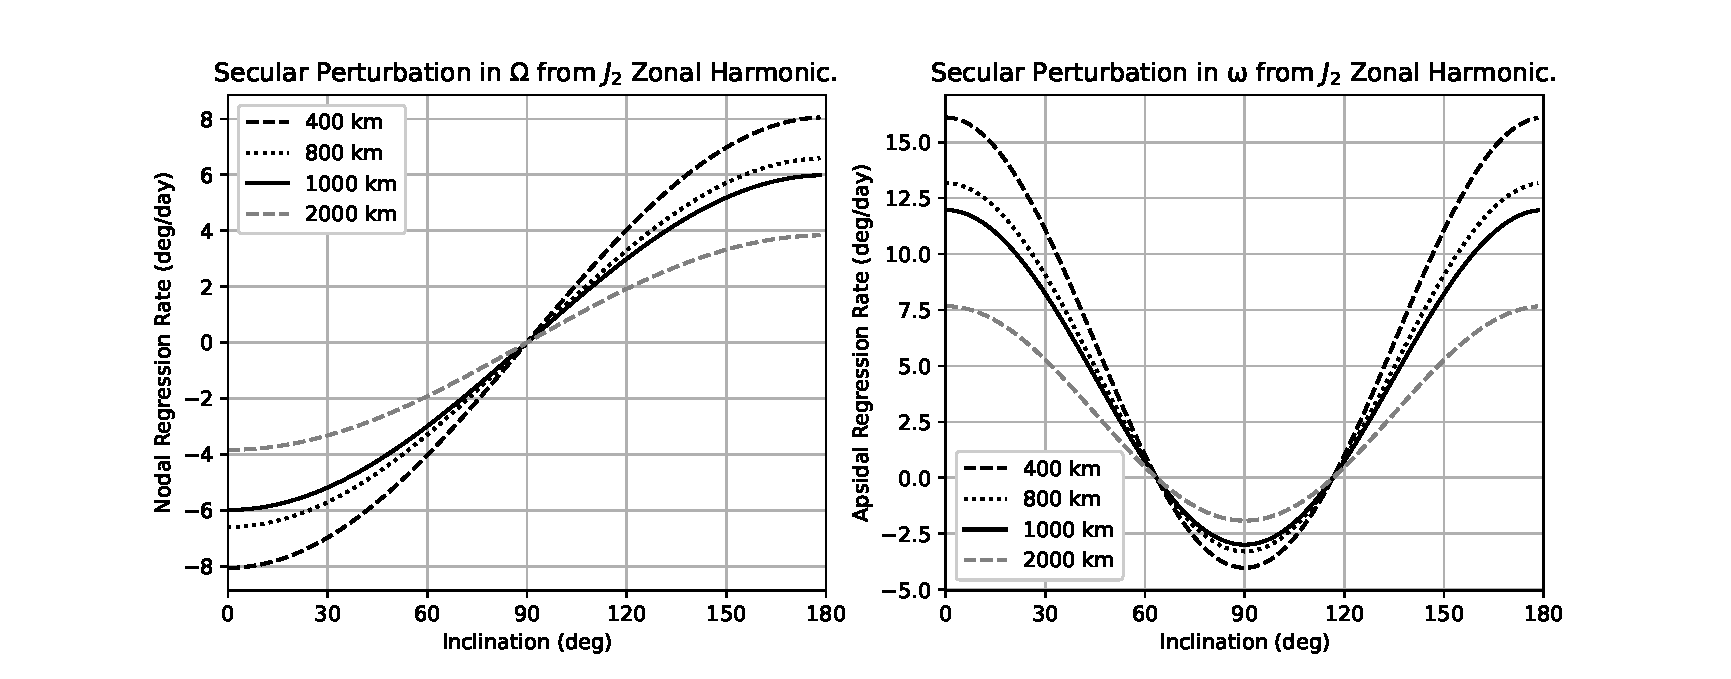
\includegraphics [angle=0, width=1\columnwidth, viewport=60 0 750 300, clip] {figures/secular_perturbation_example.eps}
    \caption{\label{fig:secular_example}Secular perturbations in $\Omega$ and $\omega$ due
      to the $J_2$ harmonic for several altitudes.
      The value $e=0.01$ is assumed for eccentricity.}
  \end {center}
\end {figure}

\subsection{Elements and Orbit State Vectors}

\newpage
\section{SGP4 Solution}
\subsection{Approximation}
\subsection{Coordinate Systems and Frames}
\subsubsection{Mean-of-Date (MoD)}
\subsubsection{True-of-Date (ToD)}
\subsubsection{True-Equator, Mean-Equinox (TEME)}
\subsubsection{Pseudo Earth-Fixed (PEF)}
\subsection{Atmospheric Drag}
\subsection{Two-Line Elements}
\subsection{Kozai Mean Elements}

\begin {thebibliography}{1}
\bibitem{brouwer}
  Brouwer - Solution of the Problem of Artificial Satellite Theory Without Drag, The Astronomical Journal, 64, No. 1274, 378-396, 1959 (\url{https://adsabs.harvard.edu/full/1959AJ.....64..378B}).
\bibitem{karttunen}
  Karttunen - Johdatus Taivaanmekaniikkaan, Ursan julkaisuja 1982, T�htitieteellinen yhdistys Ursa, 2001.
\bibitem{vonzeipel_rand}
  Hutcheson - A Basic Approach to the Use of Canonical Variables and Von Zeipel's Method in Perturbation Theory, Memorandum RM-4074-PR, the RAND Corporation, 1964.
\bibitem{astrodynamics}
  Bate, Mueller, White, Saylor, Fundamentals of Astrodynamics, 2ed, Dover, 2020
\bibitem{vallado_code}
Vallado - Companion code for Fundamentals of Astrodynamics and Applications, 2013.
\bibitem{hoots}
Hoots, Roehrich - Spacetrack Report No. 3, 1980 (\url{https://celestrak.org/NORAD/documentation/spacetrk.pdf}).
\bibitem{lane}
Lane, Hoots - General Perturbation Theories Derived from the 1965 Lane Drag Theory, Project Space Track, 1979 (\url{https://apps.dtic.mil/sti/citations/ADA081264}).
\bibitem{hoots}
Hoots, Schumacher, Glover - History of Analytical Orbit Modeling in the U.S. Space Surveillance System, Journal of Guidance, Control and Dynamics, Vol 27, No.2. 174-185 March-April 2004 (\url{https://arc.aiaa.org/doi/10.2514/1.9161}).
\bibitem{hujsak}
Hujsak - A Restricted Four Body Solution for Resonating Satellites without Drag, Project Space Track, 1979 (\url{https://apps.dtic.mil/sti/citations/ADA081263}).
\bibitem{revisit}
Vallado, Crawford, Hujsak - Revisiting Spacetrack Report No.3,  American Institute of Aeronautics and Astronautics, AIAA 2006-6753, 2006 (\url{https://celestrak.org/publications/AIAA/2006-6753/AIAA-2006-6753.pdf}).
  
  
\end {thebibliography}

\end {document}
